\documentclass{whiteboard}
\begin{document}
\begin{frame}[plain,t]
 \bbcover{OJ 10505}{Montesco vs Capuleto}{Prof. Edson Alves}{Faculdade UnB Gama}
\end{frame}

\begin{frame}[plain,t]
\vspace*{\fill}
 \bbenglish{Romeo and Juliet have finally decided to get married. But preparing the wedding party will not be so easy, as it is well-known that their respective families --the Montesco and the Capuleto-- are bloody enemies. In this problem you will have to decide which person to invite and which person not to invite, in order to prevent a slaugther.}

 \vspace{0.1in}

 \bbenglish{We have a list of $N$ people who can be invited to the party or not. For every person $i$, we have a list of his enemies: $E_1, E_2, \ldots, E_p$. The ``enemy'' relationship has the following properties:}

 \vspace{0.1in}

 \begin{description}
 \item [Anti-transitive.] \bbenglish{If $a$ is an enemy of $b$, and $b$ is an enemy of $c$, then $a$ is a friend of $c$. Also, the enemies of the friends of $a$ are his enemies, and the friends of the friends of $a$ are his friends.}
 \item [Symmetrical.] \bbenglish{If $a$ is an enemy of $b$, then $b$ is an enemy of $a$ (although it may not be indicated in his list of enemies).}
 \end{description}
\vspace*{\fill}
\end{frame}

\begin{frame}[plain,t]
\vspace*{\fill}
 \bbtext{Romeu e Julieta decidiram finalmente se casar. Mas os preparativos para a festa do casamento não serão fáceis, uma vez que é bem conhecido que suas respectivas famílias -- os Montescos e os Capuletos -- são inimigos mortais. Neste problema você deve decidir quais pessoas convidar ou não, para prevenir um massacre.}

 \vspace{0.1in}

 \bbtext{Nós temos uma listas das $N$ pessoas que podem ser convidadas para a festa ou não. Para cada pessoa $i$, nos temos uma lista de seus inimigos: $E_1, E_2, \ldots, E_p$. A relação de ``inimizade'' tem as seguintes propriedades:}

 \vspace{0.1in}

 \begin{description}
 \item [Anti-transitiva.] \bbtext{Se $a$ é um inimigo de $b$, e $b$ é um inimigo de $c$, então $a$ é amigo de $c$. Além disso, os inimigos dos amigos de $a$ são seus inimigos, e os amigos dos amigos de $a$ são seus amigos.}
 \item [Simétrica.] \bbtext{Se $a$ é inimigo de $b$, então $b$ é inimigo de $a$ (embora isto possa não estar indicado na lista de seus inimigos).}
 \end{description}
\vspace*{\fill}
\end{frame}

\begin{frame}[plain,t]
\vspace*{\fill}
 \bbenglish{One person will accept an invitation to the party if, and only if, he is invited, all his friends are invited and none of his enemies is invited. You have to find the maximum number of people that can be invited, so that all of them accept their invitation.}

 \vspace{0.1in}

 \bbenglish{For instance, if $N = 5$, and we know that: $1$ is enemy of $3$, $2$ is enemy of $1$, and $4$ is enemy of $5$, then we could invite a maximum of $3$ people. These people could be $2$, $3$ and $4$, but for this problem we only want the number of people invited.}
\vspace*{\fill}
\end{frame}

\begin{frame}[plain,t]
\vspace*{\fill}
 \bbtext{Uma pessoa aceitará o convite para a festa se, e somente se, ele foi convidado, todos os seus amigos foram convidados e nenhum de seus inimigos foi convidado. Você deve escolhar o número máximo de pessoas que podem ser convidadas, de modo que todos aceitem o convite.}

 \vspace{0.1in}

 \bbtext{Por exemplo, se $N = 5$ e nós sabemos que: $1$ é inimigo de $3$, $2$ é inimigo de $1$, e $4$ é inimigo de $5$, então nós deveríamos convidar no máximo $3$ pessoas. Estas pessoas poderiam ser $2$, $3$ e $4$, mas para este problema nos queremos apenas o número de pessoas convidadas.}
\vspace*{\fill}
\end{frame}

\begin{frame}[plain,t]
\vspace*{\fill}
 \bbbold{Input}

 \vspace{0.1in}

 \bbenglish{The first line of the input file contains the number $M$ of test cases in this file. A blank line follows this number, and a blank line is also used to separate test cases. The first line of each test case contains an integer $N$, indicating the number of people who have to be considered. You can assume that $N\leq 200$.  For each of these $N$ people, there is a line with his list of enemies. The first line contains the list of enemies of person $1$, the second line contains the list of enemies of person $2$, and so on. Each list of enemies starts with an integer $p$ (the number of known enemies of that person) and then, there are $p$ integers (the $p$ enemies of that person).  So, for example, if a person’s enemies are $5$ and $7$, his list of enemies would be: ‘\texttt{2 5 7}’.}
\vspace*{\fill}
\end{frame}

\begin{frame}[plain,t]
\vspace*{\fill}
 \bbbold{Entrada}

 \vspace{0.1in}

 \bbtext{A primeira linha da entrada contém o número $M$ de casos de teste. Uma linha em branco seguirá este número, e uma linha em branco também será usada para separar os casos de teste. A primeira linha de cada caso de teste contém um inteiro $N$, indicando o número de pessoas que foram consideradas. Você pode assumir que $N\leq 200$.  Para cada uma destas $N$ pessoas há uma linha com a lista de seus inimigos. A primeira linha contém a lista de inimigos da pessoa $1$, a segunda linha contéme a lista de inimigos da pessoa $2$, e assim por diante. Cada lista de inimigos inicia com um inteiro $p$ (o número de inimigos conhecidos daquela pessoa) e, em seguida, há $p$ inteiros (os $p$ inimigos daquela pessoa). Por exemplo, se os inimigos da pessoa são $5$ e $7$, sua lista de inimigos seria: ‘\texttt{2 5 7}’.}
\vspace*{\fill}
\end{frame}

\begin{frame}[plain,t]
\vspace*{\fill}
 \bbbold{Output}

 \vspace{0.1in}

 \bbenglish{For each test case, the output should consist of a single line containing an integer, the maximum number of people who can be invited, so that all of them accept their invitation.}
\vspace*{\fill}
\end{frame}

\begin{frame}[plain,t]
\vspace*{\fill}
 \bbbold{Saída}

 \vspace{0.1in}

 \bbtext{Para cada caso de teste a saída deverá consistir em uma única linha contendo um inteiro, o número máximo e pessoas que podem ser convidadas, de modo que todas elas aceitem o convite.}
\vspace*{\fill}
\end{frame}

\begin{frame}[plain,t]
\begin{tikzpicture}
\node[draw,opacity=0] at (0, 0) {x};
\node[draw,opacity=0] at (14, 8) {x};
 \node[anchor=west] at (0, 7) { \bbbold{Exemplo de entrada e saída} };
\end{tikzpicture}
\end{frame}

\begin{frame}[plain,t]
\begin{tikzpicture}
\node[draw,opacity=0] at (0, 0) {x};
\node[draw,opacity=0] at (14, 8) {x};
 \node[anchor=west] at (0, 7) { \bbbold{Exemplo de entrada e saída} };
 \node[anchor=west] at (1, 6) { \bbtext{3} };
\end{tikzpicture}
\end{frame}

\begin{frame}[plain,t]
\begin{tikzpicture}
\node[draw,opacity=0] at (0, 0) {x};
\node[draw,opacity=0] at (14, 8) {x};
 \node[anchor=west] at (0, 7) { \bbbold{Exemplo de entrada e saída} };
 \node[anchor=west] at (1, 6) { \bbtext{3} };
 \node at (1.25, 5) { \footnotesize \bbcomment{\# de casos de teste} };
 \draw[->,color=BBViolet] (1.25, 5.2) -- (1.25, 5.8);
\end{tikzpicture}
\end{frame}

\begin{frame}[plain,t]
\begin{tikzpicture}
\node[draw,opacity=0] at (0, 0) {x};
\node[draw,opacity=0] at (14, 8) {x};
 \node[anchor=west] at (0, 7) { \bbbold{Exemplo de entrada e saída} };
 \node[anchor=west] at (1, 6) { \bbtext{3} };
\end{tikzpicture}
\end{frame}

\begin{frame}[plain,t]
\begin{tikzpicture}
\node[draw,opacity=0] at (0, 0) {x};
\node[draw,opacity=0] at (14, 8) {x};
 \node[anchor=west] at (0, 7) { \bbbold{Exemplo de entrada e saída} };
 \node[anchor=west] at (1, 6) { \bbtext{3} };
 \node[anchor=west] at (1, 5) { \bbtext{5} };
\end{tikzpicture}
\end{frame}

\begin{frame}[plain,t]
\begin{tikzpicture}
\node[draw,opacity=0] at (0, 0) {x};
\node[draw,opacity=0] at (14, 8) {x};
 \node[anchor=west] at (0, 7) { \bbbold{Exemplo de entrada e saída} };
 \node[anchor=west] at (1, 6) { \bbtext{3} };
 \node[anchor=west] at (1, 5) { \bbtext{5} };
 \node[anchor=west] at (0.5, 4) { \footnotesize \bbcomment{\# de pessoas consideradas} };
 \draw[->,color=BBViolet] (1.25, 4.2) -- (1.25, 4.8);
\end{tikzpicture}
\end{frame}

\begin{frame}[plain,t]
\begin{tikzpicture}
\node[draw,opacity=0] at (0, 0) {x};
\node[draw,opacity=0] at (14, 8) {x};
 \node[anchor=west] at (0, 7) { \bbbold{Exemplo de entrada e saída} };
 \node[anchor=west] at (1, 6) { \bbtext{3} };
 \node[anchor=west] at (1, 5) { \bbtext{5} };
 \node[draw,very thick,circle] (A) at (6, 4) { \bbtext{1} };
 \node[draw,very thick,circle] (B) at (9, 7) { \bbtext{2} };
 \node[draw,very thick,circle] (C) at (12, 4) { \bbtext{3} };
 \node[draw,very thick,circle] (D) at (11, 1) { \bbtext{4} };
 \node[draw,very thick,circle] (E) at (7, 1) { \bbtext{5} };
\end{tikzpicture}
\end{frame}

\begin{frame}[plain,t]
\begin{tikzpicture}
\node[draw,opacity=0] at (0, 0) {x};
\node[draw,opacity=0] at (14, 8) {x};
 \node[anchor=west] at (0, 7) { \bbbold{Exemplo de entrada e saída} };
 \node[anchor=west] at (1, 6) { \bbtext{3} };
 \node[anchor=west] at (1, 5) { \bbtext{5} };
 \node[draw,very thick,circle] (A) at (6, 4) { \bbtext{1} };
 \node[draw,very thick,circle] (B) at (9, 7) { \bbtext{2} };
 \node[draw,very thick,circle] (C) at (12, 4) { \bbtext{3} };
 \node[draw,very thick,circle] (D) at (11, 1) { \bbtext{4} };
 \node[draw,very thick,circle] (E) at (7, 1) { \bbtext{5} };
 \node[anchor=west] at (1, 4.5) { \bbtext{1 3} };
\end{tikzpicture}
\end{frame}

\begin{frame}[plain,t]
\begin{tikzpicture}
\node[draw,opacity=0] at (0, 0) {x};
\node[draw,opacity=0] at (14, 8) {x};
 \node[anchor=west] at (0, 7) { \bbbold{Exemplo de entrada e saída} };
 \node[anchor=west] at (1, 6) { \bbtext{3} };
 \node[anchor=west] at (1, 5) { \bbtext{5} };
 \node[draw,very thick,circle] (A) at (6, 4) { \bbtext{1} };
 \node[draw,very thick,circle] (B) at (9, 7) { \bbtext{2} };
 \node[draw,very thick,circle] (C) at (12, 4) { \bbtext{3} };
 \node[draw,very thick,circle] (D) at (11, 1) { \bbtext{4} };
 \node[draw,very thick,circle] (E) at (7, 1) { \bbtext{5} };
 \node[anchor=west] at (1, 4.5) { \bbtext{1 3} };
 \draw[thick] (A) to (C);
\end{tikzpicture}
\end{frame}

\begin{frame}[plain,t]
\begin{tikzpicture}
\node[draw,opacity=0] at (0, 0) {x};
\node[draw,opacity=0] at (14, 8) {x};
 \node[anchor=west] at (0, 7) { \bbbold{Exemplo de entrada e saída} };
 \node[anchor=west] at (1, 6) { \bbtext{3} };
 \node[anchor=west] at (1, 5) { \bbtext{5} };
 \node[draw,very thick,circle] (A) at (6, 4) { \bbtext{1} };
 \node[draw,very thick,circle] (B) at (9, 7) { \bbtext{2} };
 \node[draw,very thick,circle] (C) at (12, 4) { \bbtext{3} };
 \node[draw,very thick,circle] (D) at (11, 1) { \bbtext{4} };
 \node[draw,very thick,circle] (E) at (7, 1) { \bbtext{5} };
 \node[anchor=west] at (1, 4.5) { \bbtext{1 3} };
 \draw[thick] (A) to (C);
 \node[anchor=west] at (1, 4.0) { \bbtext{1 1} };
\end{tikzpicture}
\end{frame}

\begin{frame}[plain,t]
\begin{tikzpicture}
\node[draw,opacity=0] at (0, 0) {x};
\node[draw,opacity=0] at (14, 8) {x};
 \node[anchor=west] at (0, 7) { \bbbold{Exemplo de entrada e saída} };
 \node[anchor=west] at (1, 6) { \bbtext{3} };
 \node[anchor=west] at (1, 5) { \bbtext{5} };
 \node[draw,very thick,circle] (A) at (6, 4) { \bbtext{1} };
 \node[draw,very thick,circle] (B) at (9, 7) { \bbtext{2} };
 \node[draw,very thick,circle] (C) at (12, 4) { \bbtext{3} };
 \node[draw,very thick,circle] (D) at (11, 1) { \bbtext{4} };
 \node[draw,very thick,circle] (E) at (7, 1) { \bbtext{5} };
 \node[anchor=west] at (1, 4.5) { \bbtext{1 3} };
 \draw[thick] (A) to (C);
 \node[anchor=west] at (1, 4.0) { \bbtext{1 1} };
 \draw[thick] (A) to (B);
\end{tikzpicture}
\end{frame}

\begin{frame}[plain,t]
\begin{tikzpicture}
\node[draw,opacity=0] at (0, 0) {x};
\node[draw,opacity=0] at (14, 8) {x};
 \node[anchor=west] at (0, 7) { \bbbold{Exemplo de entrada e saída} };
 \node[anchor=west] at (1, 6) { \bbtext{3} };
 \node[anchor=west] at (1, 5) { \bbtext{5} };
 \node[draw,very thick,circle] (A) at (6, 4) { \bbtext{1} };
 \node[draw,very thick,circle] (B) at (9, 7) { \bbtext{2} };
 \node[draw,very thick,circle] (C) at (12, 4) { \bbtext{3} };
 \node[draw,very thick,circle] (D) at (11, 1) { \bbtext{4} };
 \node[draw,very thick,circle] (E) at (7, 1) { \bbtext{5} };
 \node[anchor=west] at (1, 4.5) { \bbtext{1 3} };
 \draw[thick] (A) to (C);
 \node[anchor=west] at (1, 4.0) { \bbtext{1 1} };
 \draw[thick] (A) to (B);
 \node[anchor=west] at (1, 3.5) { \bbtext{0} };
\end{tikzpicture}
\end{frame}

\begin{frame}[plain,t]
\begin{tikzpicture}
\node[draw,opacity=0] at (0, 0) {x};
\node[draw,opacity=0] at (14, 8) {x};
 \node[anchor=west] at (0, 7) { \bbbold{Exemplo de entrada e saída} };
 \node[anchor=west] at (1, 6) { \bbtext{3} };
 \node[anchor=west] at (1, 5) { \bbtext{5} };
 \node[draw,very thick,circle] (A) at (6, 4) { \bbtext{1} };
 \node[draw,very thick,circle] (B) at (9, 7) { \bbtext{2} };
 \node[draw,very thick,circle] (C) at (12, 4) { \bbtext{3} };
 \node[draw,very thick,circle] (D) at (11, 1) { \bbtext{4} };
 \node[draw,very thick,circle] (E) at (7, 1) { \bbtext{5} };
 \node[anchor=west] at (1, 4.5) { \bbtext{1 3} };
 \draw[thick] (A) to (C);
 \node[anchor=west] at (1, 4.0) { \bbtext{1 1} };
 \draw[thick] (A) to (B);
 \node[anchor=west] at (1, 3.5) { \bbtext{0} };
 \node[anchor=west] at (1, 3.0) { \bbtext{1 5} };
\end{tikzpicture}
\end{frame}

\begin{frame}[plain,t]
\begin{tikzpicture}
\node[draw,opacity=0] at (0, 0) {x};
\node[draw,opacity=0] at (14, 8) {x};
 \node[anchor=west] at (0, 7) { \bbbold{Exemplo de entrada e saída} };
 \node[anchor=west] at (1, 6) { \bbtext{3} };
 \node[anchor=west] at (1, 5) { \bbtext{5} };
 \node[draw,very thick,circle] (A) at (6, 4) { \bbtext{1} };
 \node[draw,very thick,circle] (B) at (9, 7) { \bbtext{2} };
 \node[draw,very thick,circle] (C) at (12, 4) { \bbtext{3} };
 \node[draw,very thick,circle] (D) at (11, 1) { \bbtext{4} };
 \node[draw,very thick,circle] (E) at (7, 1) { \bbtext{5} };
 \node[anchor=west] at (1, 4.5) { \bbtext{1 3} };
 \draw[thick] (A) to (C);
 \node[anchor=west] at (1, 4.0) { \bbtext{1 1} };
 \draw[thick] (A) to (B);
 \node[anchor=west] at (1, 3.5) { \bbtext{0} };
 \node[anchor=west] at (1, 3.0) { \bbtext{1 5} };
 \draw[thick] (D) to (E);
\end{tikzpicture}
\end{frame}

\begin{frame}[plain,t]
\begin{tikzpicture}
\node[draw,opacity=0] at (0, 0) {x};
\node[draw,opacity=0] at (14, 8) {x};
 \node[anchor=west] at (0, 7) { \bbbold{Exemplo de entrada e saída} };
 \node[anchor=west] at (1, 6) { \bbtext{3} };
 \node[anchor=west] at (1, 5) { \bbtext{5} };
 \node[draw,very thick,circle] (A) at (6, 4) { \bbtext{1} };
 \node[draw,very thick,circle] (B) at (9, 7) { \bbtext{2} };
 \node[draw,very thick,circle] (C) at (12, 4) { \bbtext{3} };
 \node[draw,very thick,circle] (D) at (11, 1) { \bbtext{4} };
 \node[draw,very thick,circle] (E) at (7, 1) { \bbtext{5} };
 \node[anchor=west] at (1, 4.5) { \bbtext{1 3} };
 \draw[thick] (A) to (C);
 \node[anchor=west] at (1, 4.0) { \bbtext{1 1} };
 \draw[thick] (A) to (B);
 \node[anchor=west] at (1, 3.5) { \bbtext{0} };
 \node[anchor=west] at (1, 3.0) { \bbtext{1 5} };
 \draw[thick] (D) to (E);
 \node[anchor=west] at (1, 2.5) { \bbtext{0} };
\end{tikzpicture}
\end{frame}

\begin{frame}[plain,t]
\begin{tikzpicture}
\node[draw,opacity=0] at (0, 0) {x};
\node[draw,opacity=0] at (14, 8) {x};
 \node[anchor=west] at (0, 7) { \bbbold{Exemplo de entrada e saída} };
 \node[anchor=west] at (1, 6) { \bbtext{3} };
 \node[anchor=west] at (1, 5) { \bbtext{5} };
 \node[draw,very thick,circle] (B) at (9, 7) { \bbtext{2} };
 \node[draw,very thick,circle] (C) at (12, 4) { \bbtext{3} };
 \node[draw,very thick,circle] (D) at (11, 1) { \bbtext{4} };
 \node[draw,very thick,circle] (E) at (7, 1) { \bbtext{5} };
 \node[anchor=west] at (1, 4.5) { \bbtext{1 3} };
 \draw[thick] (A) to (C);
 \node[anchor=west] at (1, 4.0) { \bbtext{1 1} };
 \draw[thick] (A) to (B);
 \node[anchor=west] at (1, 3.5) { \bbtext{0} };
 \node[anchor=west] at (1, 3.0) { \bbtext{1 5} };
 \draw[thick] (D) to (E);
 \node[anchor=west] at (1, 2.5) { \bbtext{0} };
 \node[fill,color=BBCyan,circle] (A) at (6, 4) { \bbtext{1} };
 \node[draw,very thick,circle] (A) at (6, 4) { \bbtext{1} };
\end{tikzpicture}
\end{frame}

\begin{frame}[plain,t]
\begin{tikzpicture}
\node[draw,opacity=0] at (0, 0) {x};
\node[draw,opacity=0] at (14, 8) {x};
 \node[anchor=west] at (0, 7) { \bbbold{Exemplo de entrada e saída} };
 \node[anchor=west] at (1, 6) { \bbtext{3} };
 \node[anchor=west] at (1, 5) { \bbtext{5} };
 \node[draw,very thick,circle] (C) at (12, 4) { \bbtext{3} };
 \node[draw,very thick,circle] (D) at (11, 1) { \bbtext{4} };
 \node[draw,very thick,circle] (E) at (7, 1) { \bbtext{5} };
 \node[anchor=west] at (1, 4.5) { \bbtext{1 3} };
 \draw[thick] (A) to (C);
 \node[anchor=west] at (1, 4.0) { \bbtext{1 1} };
 \node[anchor=west] at (1, 3.5) { \bbtext{0} };
 \node[anchor=west] at (1, 3.0) { \bbtext{1 5} };
 \draw[thick] (D) to (E);
 \node[anchor=west] at (1, 2.5) { \bbtext{0} };
 \node[fill,color=BBCyan,circle] (A) at (6, 4) { \bbtext{1} };
 \node[draw,very thick,circle] (A) at (6, 4) { \bbtext{1} };
 \draw[-latex,very thick] (A) to (B);
 \node[fill,color=BBGreen,circle] (B) at (9, 7) { \bbtext{2} };
 \node[draw,very thick,circle] (B) at (9, 7) { \bbtext{2} };
\end{tikzpicture}
\end{frame}

\begin{frame}[plain,t]
\begin{tikzpicture}
\node[draw,opacity=0] at (0, 0) {x};
\node[draw,opacity=0] at (14, 8) {x};
 \node[anchor=west] at (0, 7) { \bbbold{Exemplo de entrada e saída} };
 \node[anchor=west] at (1, 6) { \bbtext{3} };
 \node[anchor=west] at (1, 5) { \bbtext{5} };
 \node[draw,very thick,circle] (D) at (11, 1) { \bbtext{4} };
 \node[draw,very thick,circle] (E) at (7, 1) { \bbtext{5} };
 \node[anchor=west] at (1, 4.5) { \bbtext{1 3} };
 \node[anchor=west] at (1, 4.0) { \bbtext{1 1} };
 \node[anchor=west] at (1, 3.5) { \bbtext{0} };
 \node[anchor=west] at (1, 3.0) { \bbtext{1 5} };
 \draw[thick] (D) to (E);
 \node[anchor=west] at (1, 2.5) { \bbtext{0} };
 \node[fill,color=BBCyan,circle] (A) at (6, 4) { \bbtext{1} };
 \node[draw,very thick,circle] (A) at (6, 4) { \bbtext{1} };
 \draw[-latex,very thick] (A) to (B);
 \node[fill,color=BBGreen,circle] (B) at (9, 7) { \bbtext{2} };
 \node[draw,very thick,circle] (B) at (9, 7) { \bbtext{2} };
 \draw[-latex,very thick] (A) to (C);
 \node[fill,color=BBGreen,circle] (C) at (12, 4) { \bbtext{3} };
 \node[draw,very thick,circle] (C) at (12, 4) { \bbtext{3} };
\end{tikzpicture}
\end{frame}

\begin{frame}[plain,t]
\begin{tikzpicture}
\node[draw,opacity=0] at (0, 0) {x};
\node[draw,opacity=0] at (14, 8) {x};
 \node[anchor=west] at (0, 7) { \bbbold{Exemplo de entrada e saída} };
 \node[anchor=west] at (1, 6) { \bbtext{3} };
 \node[anchor=west] at (1, 5) { \bbtext{5} };
 \node[draw,very thick,circle] (D) at (11, 1) { \bbtext{4} };
 \node[draw,very thick,circle] (E) at (7, 1) { \bbtext{5} };
 \node[anchor=west] at (1, 4.5) { \bbtext{1 3} };
 \node[anchor=west] at (1, 4.0) { \bbtext{1 1} };
 \node[anchor=west] at (1, 3.5) { \bbtext{0} };
 \node[anchor=west] at (1, 3.0) { \bbtext{1 5} };
 \draw[thick] (D) to (E);
 \node[anchor=west] at (1, 2.5) { \bbtext{0} };
 \node[fill,color=BBCyan,circle] (A) at (6, 4) { \bbtext{1} };
 \node[draw,very thick,circle] (A) at (6, 4) { \bbtext{1} };
 \draw[-latex,very thick] (A) to (B);
 \node[fill,color=BBGreen,circle] (B) at (9, 7) { \bbtext{2} };
 \node[draw,very thick,circle] (B) at (9, 7) { \bbtext{2} };
 \draw[-latex,very thick] (A) to (C);
 \node[fill,color=BBGreen,circle] (C) at (12, 4) { \bbtext{3} };
 \node[draw,very thick,circle] (C) at (12, 4) { \bbtext{3} };
 \node[anchor=west] (X) at (11, 7) { \bbcomment{convidados} };
 \draw[-latex, color=BBViolet] (X) to (B);
 \draw[-latex, color=BBViolet] (X) to (C);
\end{tikzpicture}
\end{frame}

\begin{frame}[plain,t]
\begin{tikzpicture}
\node[draw,opacity=0] at (0, 0) {x};
\node[draw,opacity=0] at (14, 8) {x};
 \node[anchor=west] at (0, 7) { \bbbold{Exemplo de entrada e saída} };
 \node[anchor=west] at (1, 6) { \bbtext{3} };
 \node[anchor=west] at (1, 5) { \bbtext{5} };
 \node[draw,very thick,circle] (D) at (11, 1) { \bbtext{4} };
 \node[anchor=west] at (1, 4.5) { \bbtext{1 3} };
 \node[anchor=west] at (1, 4.0) { \bbtext{1 1} };
 \node[anchor=west] at (1, 3.5) { \bbtext{0} };
 \node[anchor=west] at (1, 3.0) { \bbtext{1 5} };
 \draw[thick] (D) to (E);
 \node[anchor=west] at (1, 2.5) { \bbtext{0} };
 \node[fill,color=BBCyan,circle] (A) at (6, 4) { \bbtext{1} };
 \node[draw,very thick,circle] (A) at (6, 4) { \bbtext{1} };
 \draw[-latex,very thick] (A) to (B);
 \node[fill,color=BBGreen,circle] (B) at (9, 7) { \bbtext{2} };
 \node[draw,very thick,circle] (B) at (9, 7) { \bbtext{2} };
 \draw[-latex,very thick] (A) to (C);
 \node[fill,color=BBGreen,circle] (C) at (12, 4) { \bbtext{3} };
 \node[draw,very thick,circle] (C) at (12, 4) { \bbtext{3} };
 \node[anchor=west] (X) at (11, 7) { \bbcomment{convidados} };
 \draw[-latex, color=BBViolet] (X) to (B);
 \draw[-latex, color=BBViolet] (X) to (C);
 \node[fill,color=BBGreen,circle] (E) at (7, 1) { \bbtext{5} };
 \node[draw,very thick,circle] (E) at (7, 1) { \bbtext{5} };
\end{tikzpicture}
\end{frame}

\begin{frame}[plain,t]
\begin{tikzpicture}
\node[draw,opacity=0] at (0, 0) {x};
\node[draw,opacity=0] at (14, 8) {x};
 \node[anchor=west] at (0, 7) { \bbbold{Exemplo de entrada e saída} };
 \node[anchor=west] at (1, 6) { \bbtext{3} };
 \node[anchor=west] at (1, 5) { \bbtext{5} };
 \node[anchor=west] at (1, 4.5) { \bbtext{1 3} };
 \node[anchor=west] at (1, 4.0) { \bbtext{1 1} };
 \node[anchor=west] at (1, 3.5) { \bbtext{0} };
 \node[anchor=west] at (1, 3.0) { \bbtext{1 5} };
 \node[anchor=west] at (1, 2.5) { \bbtext{0} };
 \node[fill,color=BBCyan,circle] (A) at (6, 4) { \bbtext{1} };
 \node[draw,very thick,circle] (A) at (6, 4) { \bbtext{1} };
 \draw[-latex,very thick] (A) to (B);
 \node[fill,color=BBGreen,circle] (B) at (9, 7) { \bbtext{2} };
 \node[draw,very thick,circle] (B) at (9, 7) { \bbtext{2} };
 \draw[-latex,very thick] (A) to (C);
 \node[fill,color=BBGreen,circle] (C) at (12, 4) { \bbtext{3} };
 \node[draw,very thick,circle] (C) at (12, 4) { \bbtext{3} };
 \node[anchor=west] (X) at (11, 7) { \bbcomment{convidados} };
 \draw[-latex, color=BBViolet] (X) to (B);
 \draw[-latex, color=BBViolet] (X) to (C);
 \node[fill,color=BBGreen,circle] (E) at (7, 1) { \bbtext{5} };
 \node[draw,very thick,circle] (E) at (7, 1) { \bbtext{5} };
 \draw[latex-,very thick] (D) to (E);
 \node[fill,color=BBCyan,circle] (D) at (11, 1) { \bbtext{4} };
 \node[draw,very thick,circle] (D) at (11, 1) { \bbtext{4} };
\end{tikzpicture}
\end{frame}

\begin{frame}[plain,t]
\begin{tikzpicture}
\node[draw,opacity=0] at (0, 0) {x};
\node[draw,opacity=0] at (14, 8) {x};
 \node[anchor=west] at (0, 7) { \bbbold{Exemplo de entrada e saída} };
 \node[anchor=west] at (1, 6) { \bbtext{3} };
 \node[anchor=west] at (1, 5) { \bbtext{5} };
 \node[anchor=west] at (1, 4.5) { \bbtext{1 3} };
 \node[anchor=west] at (1, 4.0) { \bbtext{1 1} };
 \node[anchor=west] at (1, 3.5) { \bbtext{0} };
 \node[anchor=west] at (1, 3.0) { \bbtext{1 5} };
 \node[anchor=west] at (1, 2.5) { \bbtext{0} };
 \node[fill,color=BBCyan,circle] (A) at (6, 4) { \bbtext{1} };
 \node[draw,very thick,circle] (A) at (6, 4) { \bbtext{1} };
 \draw[-latex,very thick] (A) to (B);
 \node[fill,color=BBGreen,circle] (B) at (9, 7) { \bbtext{2} };
 \node[draw,very thick,circle] (B) at (9, 7) { \bbtext{2} };
 \draw[-latex,very thick] (A) to (C);
 \node[fill,color=BBGreen,circle] (C) at (12, 4) { \bbtext{3} };
 \node[draw,very thick,circle] (C) at (12, 4) { \bbtext{3} };
 \node[anchor=west] (X) at (11, 7) { \bbcomment{convidados} };
 \draw[-latex, color=BBViolet] (X) to (B);
 \draw[-latex, color=BBViolet] (X) to (C);
 \node[fill,color=BBGreen,circle] (E) at (7, 1) { \bbtext{5} };
 \node[draw,very thick,circle] (E) at (7, 1) { \bbtext{5} };
 \draw[latex-,very thick] (D) to (E);
 \node[fill,color=BBCyan,circle] (D) at (11, 1) { \bbtext{4} };
 \node[draw,very thick,circle] (D) at (11, 1) { \bbtext{4} };
 \node (Y) at (9, 3) { \bbcomment{convidado} };
 \draw[-latex, color=BBViolet] (Y) to (D);
\end{tikzpicture}
\end{frame}

\begin{frame}[plain,t]
\begin{tikzpicture}
\node[draw,opacity=0] at (0, 0) {x};
\node[draw,opacity=0] at (14, 8) {x};
 \node[anchor=west] at (0, 7) { \bbbold{Exemplo de entrada e saída} };
 \node[anchor=west] at (1, 6) { \bbtext{3} };
 \node[anchor=west] at (1, 5) { \bbtext{5} };
 \node[anchor=west] at (1, 4.5) { \bbtext{1 3} };
 \node[anchor=west] at (1, 4.0) { \bbtext{1 1} };
 \node[anchor=west] at (1, 3.5) { \bbtext{0} };
 \node[anchor=west] at (1, 3.0) { \bbtext{1 5} };
 \node[anchor=west] at (1, 2.5) { \bbtext{0} };
 \node[fill,color=BBCyan,circle] (A) at (6, 4) { \bbtext{1} };
 \node[draw,very thick,circle] (A) at (6, 4) { \bbtext{1} };
 \draw[-latex,very thick] (A) to (B);
 \node[fill,color=BBGreen,circle] (B) at (9, 7) { \bbtext{2} };
 \node[draw,very thick,circle] (B) at (9, 7) { \bbtext{2} };
 \draw[-latex,very thick] (A) to (C);
 \node[fill,color=BBGreen,circle] (C) at (12, 4) { \bbtext{3} };
 \node[draw,very thick,circle] (C) at (12, 4) { \bbtext{3} };
 \node[anchor=west] (X) at (11, 7) { \bbcomment{convidados} };
 \draw[-latex, color=BBViolet] (X) to (B);
 \draw[-latex, color=BBViolet] (X) to (C);
 \node[fill,color=BBGreen,circle] (E) at (7, 1) { \bbtext{5} };
 \node[draw,very thick,circle] (E) at (7, 1) { \bbtext{5} };
 \draw[latex-,very thick] (D) to (E);
 \node[fill,color=BBCyan,circle] (D) at (11, 1) { \bbtext{4} };
 \node[draw,very thick,circle] (D) at (11, 1) { \bbtext{4} };
 \node (Y) at (9, 3) { \bbcomment{convidado} };
 \draw[-latex, color=BBViolet] (Y) to (D);
 \draw[-latex,very thick] (1.25, 1.5) to (1.25, 2.2);
 \node at (1.25, 1.2) { \bbinfo{3} };
\end{tikzpicture}
\end{frame}

\begin{frame}[plain,t]
\begin{tikzpicture}
\node[draw,opacity=0] at (0, 0) {x};
\node[draw,opacity=0] at (14, 8) {x};
 \node[anchor=west] at (0, 7) { \bbbold{Exemplo de entrada e saída} };
 \node[anchor=west] at (1, 6) { \bbtext{3} };
\end{tikzpicture}
\end{frame}

\begin{frame}[plain,t]
\begin{tikzpicture}
\node[draw,opacity=0] at (0, 0) {x};
\node[draw,opacity=0] at (14, 8) {x};
 \node[anchor=west] at (0, 7) { \bbbold{Exemplo de entrada e saída} };
 \node[anchor=west] at (1, 6) { \bbtext{3} };
 \node[anchor=west] at (1, 5) { \bbtext{8} };
\end{tikzpicture}
\end{frame}

\begin{frame}[plain,t]
\begin{tikzpicture}
\node[draw,opacity=0] at (0, 0) {x};
\node[draw,opacity=0] at (14, 8) {x};
 \node[anchor=west] at (0, 7) { \bbbold{Exemplo de entrada e saída} };
 \node[anchor=west] at (1, 6) { \bbtext{3} };
 \node[anchor=west] at (1, 5) { \bbtext{8} };
 \node[draw,very thick,circle] (A) at (6, 3) { \bbtext{1} };
 \node[draw,very thick,circle] (B) at (6, 5) { \bbtext{2} };
 \node[draw,very thick,circle] (C) at (8, 7) { \bbtext{3} };
 \node[draw,very thick,circle] (D) at (10, 7) { \bbtext{4} };
 \node[draw,very thick,circle] (E) at (12, 5) { \bbtext{5} };
 \node[draw,very thick,circle] (F) at (12, 3) { \bbtext{6} };
 \node[draw,very thick,circle] (G) at (10, 1) { \bbtext{7} };
 \node[draw,very thick,circle] (H) at (8, 1) { \bbtext{8} };
\end{tikzpicture}
\end{frame}

\begin{frame}[plain,t]
\begin{tikzpicture}
\node[draw,opacity=0] at (0, 0) {x};
\node[draw,opacity=0] at (14, 8) {x};
 \node[anchor=west] at (0, 7) { \bbbold{Exemplo de entrada e saída} };
 \node[anchor=west] at (1, 6) { \bbtext{3} };
 \node[anchor=west] at (1, 5) { \bbtext{8} };
 \node[draw,very thick,circle] (A) at (6, 3) { \bbtext{1} };
 \node[draw,very thick,circle] (B) at (6, 5) { \bbtext{2} };
 \node[draw,very thick,circle] (C) at (8, 7) { \bbtext{3} };
 \node[draw,very thick,circle] (D) at (10, 7) { \bbtext{4} };
 \node[draw,very thick,circle] (E) at (12, 5) { \bbtext{5} };
 \node[draw,very thick,circle] (F) at (12, 3) { \bbtext{6} };
 \node[draw,very thick,circle] (G) at (10, 1) { \bbtext{7} };
 \node[draw,very thick,circle] (H) at (8, 1) { \bbtext{8} };
 \node[anchor=west] at (1, 4.5) { \bbtext{2 4 5} };
\end{tikzpicture}
\end{frame}

\begin{frame}[plain,t]
\begin{tikzpicture}
\node[draw,opacity=0] at (0, 0) {x};
\node[draw,opacity=0] at (14, 8) {x};
 \node[anchor=west] at (0, 7) { \bbbold{Exemplo de entrada e saída} };
 \node[anchor=west] at (1, 6) { \bbtext{3} };
 \node[anchor=west] at (1, 5) { \bbtext{8} };
 \node[draw,very thick,circle] (A) at (6, 3) { \bbtext{1} };
 \node[draw,very thick,circle] (B) at (6, 5) { \bbtext{2} };
 \node[draw,very thick,circle] (C) at (8, 7) { \bbtext{3} };
 \node[draw,very thick,circle] (D) at (10, 7) { \bbtext{4} };
 \node[draw,very thick,circle] (E) at (12, 5) { \bbtext{5} };
 \node[draw,very thick,circle] (F) at (12, 3) { \bbtext{6} };
 \node[draw,very thick,circle] (G) at (10, 1) { \bbtext{7} };
 \node[draw,very thick,circle] (H) at (8, 1) { \bbtext{8} };
 \node[anchor=west] at (1, 4.5) { \bbtext{2 4 5} };
 \draw[thick] (A) to (D);
 \draw[thick] (A) to (E);
\end{tikzpicture}
\end{frame}

\begin{frame}[plain,t]
\begin{tikzpicture}
\node[draw,opacity=0] at (0, 0) {x};
\node[draw,opacity=0] at (14, 8) {x};
 \node[anchor=west] at (0, 7) { \bbbold{Exemplo de entrada e saída} };
 \node[anchor=west] at (1, 6) { \bbtext{3} };
 \node[anchor=west] at (1, 5) { \bbtext{8} };
 \node[draw,very thick,circle] (A) at (6, 3) { \bbtext{1} };
 \node[draw,very thick,circle] (B) at (6, 5) { \bbtext{2} };
 \node[draw,very thick,circle] (C) at (8, 7) { \bbtext{3} };
 \node[draw,very thick,circle] (D) at (10, 7) { \bbtext{4} };
 \node[draw,very thick,circle] (E) at (12, 5) { \bbtext{5} };
 \node[draw,very thick,circle] (F) at (12, 3) { \bbtext{6} };
 \node[draw,very thick,circle] (G) at (10, 1) { \bbtext{7} };
 \node[draw,very thick,circle] (H) at (8, 1) { \bbtext{8} };
 \node[anchor=west] at (1, 4.5) { \bbtext{2 4 5} };
 \draw[thick] (A) to (D);
 \draw[thick] (A) to (E);
 \node[anchor=west] at (1, 4.0) { \bbtext{2 1 3} };
\end{tikzpicture}
\end{frame}

\begin{frame}[plain,t]
\begin{tikzpicture}
\node[draw,opacity=0] at (0, 0) {x};
\node[draw,opacity=0] at (14, 8) {x};
 \node[anchor=west] at (0, 7) { \bbbold{Exemplo de entrada e saída} };
 \node[anchor=west] at (1, 6) { \bbtext{3} };
 \node[anchor=west] at (1, 5) { \bbtext{8} };
 \node[draw,very thick,circle] (A) at (6, 3) { \bbtext{1} };
 \node[draw,very thick,circle] (B) at (6, 5) { \bbtext{2} };
 \node[draw,very thick,circle] (C) at (8, 7) { \bbtext{3} };
 \node[draw,very thick,circle] (D) at (10, 7) { \bbtext{4} };
 \node[draw,very thick,circle] (E) at (12, 5) { \bbtext{5} };
 \node[draw,very thick,circle] (F) at (12, 3) { \bbtext{6} };
 \node[draw,very thick,circle] (G) at (10, 1) { \bbtext{7} };
 \node[draw,very thick,circle] (H) at (8, 1) { \bbtext{8} };
 \node[anchor=west] at (1, 4.5) { \bbtext{2 4 5} };
 \draw[thick] (A) to (D);
 \draw[thick] (A) to (E);
 \node[anchor=west] at (1, 4.0) { \bbtext{2 1 3} };
 \draw[thick] (B) to (A);
 \draw[thick] (B) to (C);
\end{tikzpicture}
\end{frame}

\begin{frame}[plain,t]
\begin{tikzpicture}
\node[draw,opacity=0] at (0, 0) {x};
\node[draw,opacity=0] at (14, 8) {x};
 \node[anchor=west] at (0, 7) { \bbbold{Exemplo de entrada e saída} };
 \node[anchor=west] at (1, 6) { \bbtext{3} };
 \node[anchor=west] at (1, 5) { \bbtext{8} };
 \node[draw,very thick,circle] (A) at (6, 3) { \bbtext{1} };
 \node[draw,very thick,circle] (B) at (6, 5) { \bbtext{2} };
 \node[draw,very thick,circle] (C) at (8, 7) { \bbtext{3} };
 \node[draw,very thick,circle] (D) at (10, 7) { \bbtext{4} };
 \node[draw,very thick,circle] (E) at (12, 5) { \bbtext{5} };
 \node[draw,very thick,circle] (F) at (12, 3) { \bbtext{6} };
 \node[draw,very thick,circle] (G) at (10, 1) { \bbtext{7} };
 \node[draw,very thick,circle] (H) at (8, 1) { \bbtext{8} };
 \node[anchor=west] at (1, 4.5) { \bbtext{2 4 5} };
 \draw[thick] (A) to (D);
 \draw[thick] (A) to (E);
 \node[anchor=west] at (1, 4.0) { \bbtext{2 1 3} };
 \draw[thick] (B) to (A);
 \draw[thick] (B) to (C);
 \node[anchor=west] at (1, 3.5) { \bbtext{0} };
 \node[anchor=west] at (1, 3.0) { \bbtext{0} };
 \node[anchor=west] at (1, 2.5) { \bbtext{0} };
\end{tikzpicture}
\end{frame}

\begin{frame}[plain,t]
\begin{tikzpicture}
\node[draw,opacity=0] at (0, 0) {x};
\node[draw,opacity=0] at (14, 8) {x};
 \node[anchor=west] at (0, 7) { \bbbold{Exemplo de entrada e saída} };
 \node[anchor=west] at (1, 6) { \bbtext{3} };
 \node[anchor=west] at (1, 5) { \bbtext{8} };
 \node[draw,very thick,circle] (A) at (6, 3) { \bbtext{1} };
 \node[draw,very thick,circle] (B) at (6, 5) { \bbtext{2} };
 \node[draw,very thick,circle] (C) at (8, 7) { \bbtext{3} };
 \node[draw,very thick,circle] (D) at (10, 7) { \bbtext{4} };
 \node[draw,very thick,circle] (E) at (12, 5) { \bbtext{5} };
 \node[draw,very thick,circle] (F) at (12, 3) { \bbtext{6} };
 \node[draw,very thick,circle] (G) at (10, 1) { \bbtext{7} };
 \node[draw,very thick,circle] (H) at (8, 1) { \bbtext{8} };
 \node[anchor=west] at (1, 4.5) { \bbtext{2 4 5} };
 \draw[thick] (A) to (D);
 \draw[thick] (A) to (E);
 \node[anchor=west] at (1, 4.0) { \bbtext{2 1 3} };
 \draw[thick] (B) to (A);
 \draw[thick] (B) to (C);
 \node[anchor=west] at (1, 3.5) { \bbtext{0} };
 \node[anchor=west] at (1, 3.0) { \bbtext{0} };
 \node[anchor=west] at (1, 2.5) { \bbtext{0} };
 \node[anchor=west] at (1, 2.0) { \bbtext{1 3} };
\end{tikzpicture}
\end{frame}

\begin{frame}[plain,t]
\begin{tikzpicture}
\node[draw,opacity=0] at (0, 0) {x};
\node[draw,opacity=0] at (14, 8) {x};
 \node[anchor=west] at (0, 7) { \bbbold{Exemplo de entrada e saída} };
 \node[anchor=west] at (1, 6) { \bbtext{3} };
 \node[anchor=west] at (1, 5) { \bbtext{8} };
 \node[draw,very thick,circle] (A) at (6, 3) { \bbtext{1} };
 \node[draw,very thick,circle] (B) at (6, 5) { \bbtext{2} };
 \node[draw,very thick,circle] (C) at (8, 7) { \bbtext{3} };
 \node[draw,very thick,circle] (D) at (10, 7) { \bbtext{4} };
 \node[draw,very thick,circle] (E) at (12, 5) { \bbtext{5} };
 \node[draw,very thick,circle] (F) at (12, 3) { \bbtext{6} };
 \node[draw,very thick,circle] (G) at (10, 1) { \bbtext{7} };
 \node[draw,very thick,circle] (H) at (8, 1) { \bbtext{8} };
 \node[anchor=west] at (1, 4.5) { \bbtext{2 4 5} };
 \draw[thick] (A) to (D);
 \draw[thick] (A) to (E);
 \node[anchor=west] at (1, 4.0) { \bbtext{2 1 3} };
 \draw[thick] (B) to (A);
 \draw[thick] (B) to (C);
 \node[anchor=west] at (1, 3.5) { \bbtext{0} };
 \node[anchor=west] at (1, 3.0) { \bbtext{0} };
 \node[anchor=west] at (1, 2.5) { \bbtext{0} };
 \node[anchor=west] at (1, 2.0) { \bbtext{1 3} };
 \draw[thick] (F) to (C);
\end{tikzpicture}
\end{frame}

\begin{frame}[plain,t]
\begin{tikzpicture}
\node[draw,opacity=0] at (0, 0) {x};
\node[draw,opacity=0] at (14, 8) {x};
 \node[anchor=west] at (0, 7) { \bbbold{Exemplo de entrada e saída} };
 \node[anchor=west] at (1, 6) { \bbtext{3} };
 \node[anchor=west] at (1, 5) { \bbtext{8} };
 \node[draw,very thick,circle] (A) at (6, 3) { \bbtext{1} };
 \node[draw,very thick,circle] (B) at (6, 5) { \bbtext{2} };
 \node[draw,very thick,circle] (C) at (8, 7) { \bbtext{3} };
 \node[draw,very thick,circle] (D) at (10, 7) { \bbtext{4} };
 \node[draw,very thick,circle] (E) at (12, 5) { \bbtext{5} };
 \node[draw,very thick,circle] (F) at (12, 3) { \bbtext{6} };
 \node[draw,very thick,circle] (G) at (10, 1) { \bbtext{7} };
 \node[draw,very thick,circle] (H) at (8, 1) { \bbtext{8} };
 \node[anchor=west] at (1, 4.5) { \bbtext{2 4 5} };
 \draw[thick] (A) to (D);
 \draw[thick] (A) to (E);
 \node[anchor=west] at (1, 4.0) { \bbtext{2 1 3} };
 \draw[thick] (B) to (A);
 \draw[thick] (B) to (C);
 \node[anchor=west] at (1, 3.5) { \bbtext{0} };
 \node[anchor=west] at (1, 3.0) { \bbtext{0} };
 \node[anchor=west] at (1, 2.5) { \bbtext{0} };
 \node[anchor=west] at (1, 2.0) { \bbtext{1 3} };
 \draw[thick] (F) to (C);
 \node[anchor=west] at (1, 1.5) { \bbtext{0} };
\end{tikzpicture}
\end{frame}

\begin{frame}[plain,t]
\begin{tikzpicture}
\node[draw,opacity=0] at (0, 0) {x};
\node[draw,opacity=0] at (14, 8) {x};
 \node[anchor=west] at (0, 7) { \bbbold{Exemplo de entrada e saída} };
 \node[anchor=west] at (1, 6) { \bbtext{3} };
 \node[anchor=west] at (1, 5) { \bbtext{8} };
 \node[draw,very thick,circle] (A) at (6, 3) { \bbtext{1} };
 \node[draw,very thick,circle] (B) at (6, 5) { \bbtext{2} };
 \node[draw,very thick,circle] (C) at (8, 7) { \bbtext{3} };
 \node[draw,very thick,circle] (D) at (10, 7) { \bbtext{4} };
 \node[draw,very thick,circle] (E) at (12, 5) { \bbtext{5} };
 \node[draw,very thick,circle] (F) at (12, 3) { \bbtext{6} };
 \node[draw,very thick,circle] (G) at (10, 1) { \bbtext{7} };
 \node[draw,very thick,circle] (H) at (8, 1) { \bbtext{8} };
 \node[anchor=west] at (1, 4.5) { \bbtext{2 4 5} };
 \draw[thick] (A) to (D);
 \draw[thick] (A) to (E);
 \node[anchor=west] at (1, 4.0) { \bbtext{2 1 3} };
 \draw[thick] (B) to (A);
 \draw[thick] (B) to (C);
 \node[anchor=west] at (1, 3.5) { \bbtext{0} };
 \node[anchor=west] at (1, 3.0) { \bbtext{0} };
 \node[anchor=west] at (1, 2.5) { \bbtext{0} };
 \node[anchor=west] at (1, 2.0) { \bbtext{1 3} };
 \draw[thick] (F) to (C);
 \node[anchor=west] at (1, 1.5) { \bbtext{0} };
 \node[anchor=west] at (1, 1.0) { \bbtext{1 5} };
\end{tikzpicture}
\end{frame}

\begin{frame}[plain,t]
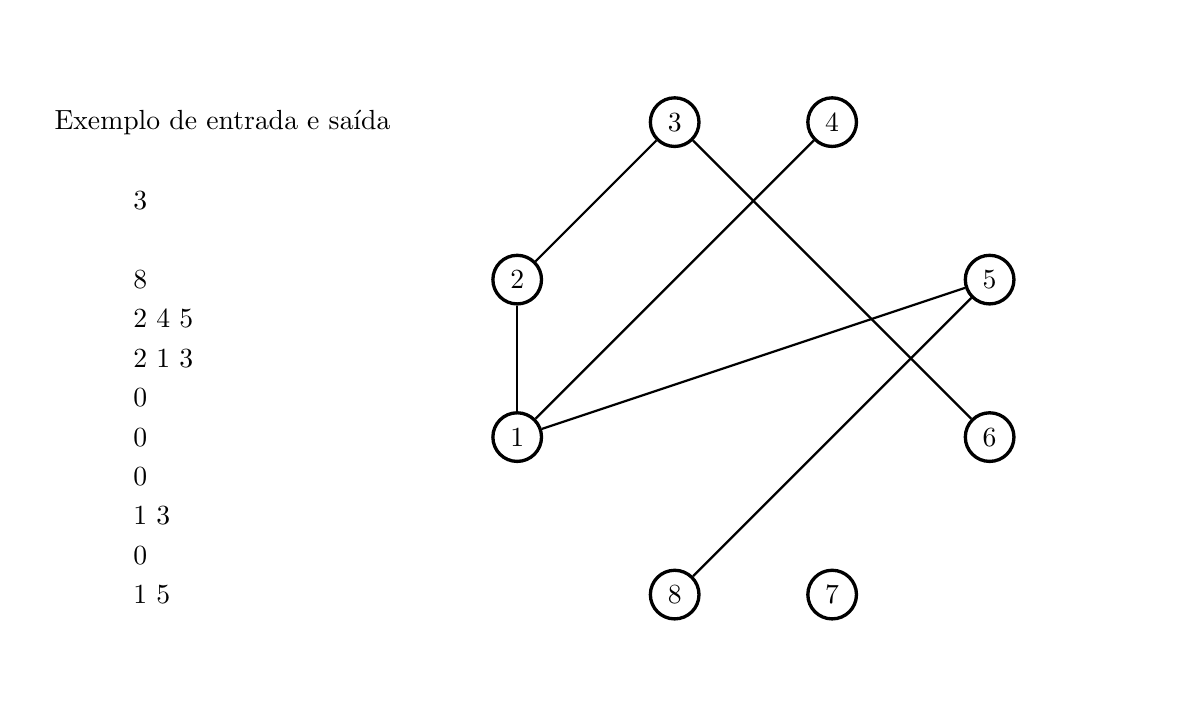
\begin{tikzpicture}
\node[draw,opacity=0] at (0, 0) {x};
\node[draw,opacity=0] at (14, 8) {x};
 \node[anchor=west] at (0, 7) { \bbbold{Exemplo de entrada e saída} };
 \node[anchor=west] at (1, 6) { \bbtext{3} };
 \node[anchor=west] at (1, 5) { \bbtext{8} };
 \node[draw,very thick,circle] (A) at (6, 3) { \bbtext{1} };
 \node[draw,very thick,circle] (B) at (6, 5) { \bbtext{2} };
 \node[draw,very thick,circle] (C) at (8, 7) { \bbtext{3} };
 \node[draw,very thick,circle] (D) at (10, 7) { \bbtext{4} };
 \node[draw,very thick,circle] (E) at (12, 5) { \bbtext{5} };
 \node[draw,very thick,circle] (F) at (12, 3) { \bbtext{6} };
 \node[draw,very thick,circle] (G) at (10, 1) { \bbtext{7} };
 \node[draw,very thick,circle] (H) at (8, 1) { \bbtext{8} };
 \node[anchor=west] at (1, 4.5) { \bbtext{2 4 5} };
 \draw[thick] (A) to (D);
 \draw[thick] (A) to (E);
 \node[anchor=west] at (1, 4.0) { \bbtext{2 1 3} };
 \draw[thick] (B) to (A);
 \draw[thick] (B) to (C);
 \node[anchor=west] at (1, 3.5) { \bbtext{0} };
 \node[anchor=west] at (1, 3.0) { \bbtext{0} };
 \node[anchor=west] at (1, 2.5) { \bbtext{0} };
 \node[anchor=west] at (1, 2.0) { \bbtext{1 3} };
 \draw[thick] (F) to (C);
 \node[anchor=west] at (1, 1.5) { \bbtext{0} };
 \node[anchor=west] at (1, 1.0) { \bbtext{1 5} };
 \draw[thick] (H) to (E);
\end{tikzpicture}
\end{frame}

\begin{frame}[plain,t]
\begin{tikzpicture}
\node[draw,opacity=0] at (0, 0) {x};
\node[draw,opacity=0] at (14, 8) {x};
 \node[anchor=west] at (0, 7) { \bbbold{Exemplo de entrada e saída} };
 \node[anchor=west] at (1, 6) { \bbtext{3} };
 \node[anchor=west] at (1, 5) { \bbtext{8} };
 \node[draw,very thick,circle] (B) at (6, 5) { \bbtext{2} };
 \node[draw,very thick,circle] (C) at (8, 7) { \bbtext{3} };
 \node[draw,very thick,circle] (D) at (10, 7) { \bbtext{4} };
 \node[draw,very thick,circle] (E) at (12, 5) { \bbtext{5} };
 \node[draw,very thick,circle] (F) at (12, 3) { \bbtext{6} };
 \node[draw,very thick,circle] (G) at (10, 1) { \bbtext{7} };
 \node[draw,very thick,circle] (H) at (8, 1) { \bbtext{8} };
 \node[anchor=west] at (1, 4.5) { \bbtext{2 4 5} };
 \draw[thick] (A) to (D);
 \draw[thick] (A) to (E);
 \node[anchor=west] at (1, 4.0) { \bbtext{2 1 3} };
 \draw[thick] (B) to (A);
 \draw[thick] (B) to (C);
 \node[anchor=west] at (1, 3.5) { \bbtext{0} };
 \node[anchor=west] at (1, 3.0) { \bbtext{0} };
 \node[anchor=west] at (1, 2.5) { \bbtext{0} };
 \node[anchor=west] at (1, 2.0) { \bbtext{1 3} };
 \draw[thick] (F) to (C);
 \node[anchor=west] at (1, 1.5) { \bbtext{0} };
 \node[anchor=west] at (1, 1.0) { \bbtext{1 5} };
 \draw[thick] (H) to (E);
 \node[fill,color=BBCyan,circle] (A) at (6, 3) { \bbtext{1} };
 \node[draw,very thick,circle] (A) at (6, 3) { \bbtext{1} };
\end{tikzpicture}
\end{frame}

\begin{frame}[plain,t]
\begin{tikzpicture}
\node[draw,opacity=0] at (0, 0) {x};
\node[draw,opacity=0] at (14, 8) {x};
 \node[anchor=west] at (0, 7) { \bbbold{Exemplo de entrada e saída} };
 \node[anchor=west] at (1, 6) { \bbtext{3} };
 \node[anchor=west] at (1, 5) { \bbtext{8} };
 \node[draw,very thick,circle] (C) at (8, 7) { \bbtext{3} };
 \node[draw,very thick,circle] (D) at (10, 7) { \bbtext{4} };
 \node[draw,very thick,circle] (E) at (12, 5) { \bbtext{5} };
 \node[draw,very thick,circle] (F) at (12, 3) { \bbtext{6} };
 \node[draw,very thick,circle] (G) at (10, 1) { \bbtext{7} };
 \node[draw,very thick,circle] (H) at (8, 1) { \bbtext{8} };
 \node[anchor=west] at (1, 4.5) { \bbtext{2 4 5} };
 \draw[thick] (A) to (D);
 \draw[thick] (A) to (E);
 \node[anchor=west] at (1, 4.0) { \bbtext{2 1 3} };
 \draw[thick] (B) to (C);
 \node[anchor=west] at (1, 3.5) { \bbtext{0} };
 \node[anchor=west] at (1, 3.0) { \bbtext{0} };
 \node[anchor=west] at (1, 2.5) { \bbtext{0} };
 \node[anchor=west] at (1, 2.0) { \bbtext{1 3} };
 \draw[thick] (F) to (C);
 \node[anchor=west] at (1, 1.5) { \bbtext{0} };
 \node[anchor=west] at (1, 1.0) { \bbtext{1 5} };
 \draw[thick] (H) to (E);
 \node[fill,color=BBCyan,circle] (A) at (6, 3) { \bbtext{1} };
 \node[draw,very thick,circle] (A) at (6, 3) { \bbtext{1} };
 \node[fill,color=BBGreen,circle] (B) at (6, 5) { \bbtext{2} };
 \node[draw,very thick,circle] (B) at (6, 5) { \bbtext{2} };
 \draw[latex-,very thick] (B) to (A);
\end{tikzpicture}
\end{frame}

\begin{frame}[plain,t]
\begin{tikzpicture}
\node[draw,opacity=0] at (0, 0) {x};
\node[draw,opacity=0] at (14, 8) {x};
 \node[anchor=west] at (0, 7) { \bbbold{Exemplo de entrada e saída} };
 \node[anchor=west] at (1, 6) { \bbtext{3} };
 \node[anchor=west] at (1, 5) { \bbtext{8} };
 \node[draw,very thick,circle] (D) at (10, 7) { \bbtext{4} };
 \node[draw,very thick,circle] (E) at (12, 5) { \bbtext{5} };
 \node[draw,very thick,circle] (F) at (12, 3) { \bbtext{6} };
 \node[draw,very thick,circle] (G) at (10, 1) { \bbtext{7} };
 \node[draw,very thick,circle] (H) at (8, 1) { \bbtext{8} };
 \node[anchor=west] at (1, 4.5) { \bbtext{2 4 5} };
 \draw[thick] (A) to (D);
 \draw[thick] (A) to (E);
 \node[anchor=west] at (1, 4.0) { \bbtext{2 1 3} };
 \node[anchor=west] at (1, 3.5) { \bbtext{0} };
 \node[anchor=west] at (1, 3.0) { \bbtext{0} };
 \node[anchor=west] at (1, 2.5) { \bbtext{0} };
 \node[anchor=west] at (1, 2.0) { \bbtext{1 3} };
 \draw[thick] (F) to (C);
 \node[anchor=west] at (1, 1.5) { \bbtext{0} };
 \node[anchor=west] at (1, 1.0) { \bbtext{1 5} };
 \draw[thick] (H) to (E);
 \node[fill,color=BBCyan,circle] (A) at (6, 3) { \bbtext{1} };
 \node[draw,very thick,circle] (A) at (6, 3) { \bbtext{1} };
 \node[fill,color=BBGreen,circle] (B) at (6, 5) { \bbtext{2} };
 \node[draw,very thick,circle] (B) at (6, 5) { \bbtext{2} };
 \draw[latex-,very thick] (B) to (A);
 \node[fill,color=BBCyan,circle] (C) at (8, 7) { \bbtext{3} };
 \node[draw,very thick,circle] (C) at (8, 7) { \bbtext{3} };
 \draw[-latex,very thick] (B) to (C);
\end{tikzpicture}
\end{frame}

\begin{frame}[plain,t]
\begin{tikzpicture}
\node[draw,opacity=0] at (0, 0) {x};
\node[draw,opacity=0] at (14, 8) {x};
 \node[anchor=west] at (0, 7) { \bbbold{Exemplo de entrada e saída} };
 \node[anchor=west] at (1, 6) { \bbtext{3} };
 \node[anchor=west] at (1, 5) { \bbtext{8} };
 \node[draw,very thick,circle] (D) at (10, 7) { \bbtext{4} };
 \node[draw,very thick,circle] (E) at (12, 5) { \bbtext{5} };
 \node[draw,very thick,circle] (G) at (10, 1) { \bbtext{7} };
 \node[draw,very thick,circle] (H) at (8, 1) { \bbtext{8} };
 \node[anchor=west] at (1, 4.5) { \bbtext{2 4 5} };
 \draw[thick] (A) to (D);
 \draw[thick] (A) to (E);
 \node[anchor=west] at (1, 4.0) { \bbtext{2 1 3} };
 \node[anchor=west] at (1, 3.5) { \bbtext{0} };
 \node[anchor=west] at (1, 3.0) { \bbtext{0} };
 \node[anchor=west] at (1, 2.5) { \bbtext{0} };
 \node[anchor=west] at (1, 2.0) { \bbtext{1 3} };
 \node[anchor=west] at (1, 1.5) { \bbtext{0} };
 \node[anchor=west] at (1, 1.0) { \bbtext{1 5} };
 \draw[thick] (H) to (E);
 \node[fill,color=BBCyan,circle] (A) at (6, 3) { \bbtext{1} };
 \node[draw,very thick,circle] (A) at (6, 3) { \bbtext{1} };
 \node[fill,color=BBGreen,circle] (B) at (6, 5) { \bbtext{2} };
 \node[draw,very thick,circle] (B) at (6, 5) { \bbtext{2} };
 \draw[latex-,very thick] (B) to (A);
 \node[fill,color=BBCyan,circle] (C) at (8, 7) { \bbtext{3} };
 \node[draw,very thick,circle] (C) at (8, 7) { \bbtext{3} };
 \draw[-latex,very thick] (B) to (C);
 \node[fill,color=BBGreen,circle] (F) at (12, 3) { \bbtext{6} };
 \node[draw,very thick,circle] (F) at (12, 3) { \bbtext{6} };
 \draw[latex-,very thick] (F) to (C);
\end{tikzpicture}
\end{frame}

\begin{frame}[plain,t]
\begin{tikzpicture}
\node[draw,opacity=0] at (0, 0) {x};
\node[draw,opacity=0] at (14, 8) {x};
 \node[anchor=west] at (0, 7) { \bbbold{Exemplo de entrada e saída} };
 \node[anchor=west] at (1, 6) { \bbtext{3} };
 \node[anchor=west] at (1, 5) { \bbtext{8} };
 \node[draw,very thick,circle] (E) at (12, 5) { \bbtext{5} };
 \node[draw,very thick,circle] (G) at (10, 1) { \bbtext{7} };
 \node[draw,very thick,circle] (H) at (8, 1) { \bbtext{8} };
 \node[anchor=west] at (1, 4.5) { \bbtext{2 4 5} };
 \draw[thick] (A) to (E);
 \node[anchor=west] at (1, 4.0) { \bbtext{2 1 3} };
 \node[anchor=west] at (1, 3.5) { \bbtext{0} };
 \node[anchor=west] at (1, 3.0) { \bbtext{0} };
 \node[anchor=west] at (1, 2.5) { \bbtext{0} };
 \node[anchor=west] at (1, 2.0) { \bbtext{1 3} };
 \node[anchor=west] at (1, 1.5) { \bbtext{0} };
 \node[anchor=west] at (1, 1.0) { \bbtext{1 5} };
 \draw[thick] (H) to (E);
 \node[fill,color=BBCyan,circle] (A) at (6, 3) { \bbtext{1} };
 \node[draw,very thick,circle] (A) at (6, 3) { \bbtext{1} };
 \node[fill,color=BBGreen,circle] (B) at (6, 5) { \bbtext{2} };
 \node[draw,very thick,circle] (B) at (6, 5) { \bbtext{2} };
 \draw[latex-,very thick] (B) to (A);
 \node[fill,color=BBCyan,circle] (C) at (8, 7) { \bbtext{3} };
 \node[draw,very thick,circle] (C) at (8, 7) { \bbtext{3} };
 \draw[-latex,very thick] (B) to (C);
 \node[fill,color=BBGreen,circle] (F) at (12, 3) { \bbtext{6} };
 \node[draw,very thick,circle] (F) at (12, 3) { \bbtext{6} };
 \draw[latex-,very thick] (F) to (C);
 \node[fill,color=BBGreen,circle] (D) at (10, 7) { \bbtext{4} };
 \node[draw,very thick,circle] (D) at (10, 7) { \bbtext{4} };
 \draw[-latex,very thick] (A) to (D);
\end{tikzpicture}
\end{frame}

\begin{frame}[plain,t]
\begin{tikzpicture}
\node[draw,opacity=0] at (0, 0) {x};
\node[draw,opacity=0] at (14, 8) {x};
 \node[anchor=west] at (0, 7) { \bbbold{Exemplo de entrada e saída} };
 \node[anchor=west] at (1, 6) { \bbtext{3} };
 \node[anchor=west] at (1, 5) { \bbtext{8} };
 \node[draw,very thick,circle] (G) at (10, 1) { \bbtext{7} };
 \node[draw,very thick,circle] (H) at (8, 1) { \bbtext{8} };
 \node[anchor=west] at (1, 4.5) { \bbtext{2 4 5} };
 \node[anchor=west] at (1, 4.0) { \bbtext{2 1 3} };
 \node[anchor=west] at (1, 3.5) { \bbtext{0} };
 \node[anchor=west] at (1, 3.0) { \bbtext{0} };
 \node[anchor=west] at (1, 2.5) { \bbtext{0} };
 \node[anchor=west] at (1, 2.0) { \bbtext{1 3} };
 \node[anchor=west] at (1, 1.5) { \bbtext{0} };
 \node[anchor=west] at (1, 1.0) { \bbtext{1 5} };
 \draw[thick] (H) to (E);
 \node[fill,color=BBCyan,circle] (A) at (6, 3) { \bbtext{1} };
 \node[draw,very thick,circle] (A) at (6, 3) { \bbtext{1} };
 \node[fill,color=BBGreen,circle] (B) at (6, 5) { \bbtext{2} };
 \node[draw,very thick,circle] (B) at (6, 5) { \bbtext{2} };
 \draw[latex-,very thick] (B) to (A);
 \node[fill,color=BBCyan,circle] (C) at (8, 7) { \bbtext{3} };
 \node[draw,very thick,circle] (C) at (8, 7) { \bbtext{3} };
 \draw[-latex,very thick] (B) to (C);
 \node[fill,color=BBGreen,circle] (F) at (12, 3) { \bbtext{6} };
 \node[draw,very thick,circle] (F) at (12, 3) { \bbtext{6} };
 \draw[latex-,very thick] (F) to (C);
 \node[fill,color=BBGreen,circle] (D) at (10, 7) { \bbtext{4} };
 \node[draw,very thick,circle] (D) at (10, 7) { \bbtext{4} };
 \draw[-latex,very thick] (A) to (D);
 \node[fill,color=BBGreen,circle] (E) at (12, 5) { \bbtext{5} };
 \node[draw,very thick,circle] (E) at (12, 5) { \bbtext{5} };
 \draw[-latex,very thick] (A) to (E);
\end{tikzpicture}
\end{frame}

\begin{frame}[plain,t]
\begin{tikzpicture}
\node[draw,opacity=0] at (0, 0) {x};
\node[draw,opacity=0] at (14, 8) {x};
 \node[anchor=west] at (0, 7) { \bbbold{Exemplo de entrada e saída} };
 \node[anchor=west] at (1, 6) { \bbtext{3} };
 \node[anchor=west] at (1, 5) { \bbtext{8} };
 \node[draw,very thick,circle] (G) at (10, 1) { \bbtext{7} };
 \node[anchor=west] at (1, 4.5) { \bbtext{2 4 5} };
 \node[anchor=west] at (1, 4.0) { \bbtext{2 1 3} };
 \node[anchor=west] at (1, 3.5) { \bbtext{0} };
 \node[anchor=west] at (1, 3.0) { \bbtext{0} };
 \node[anchor=west] at (1, 2.5) { \bbtext{0} };
 \node[anchor=west] at (1, 2.0) { \bbtext{1 3} };
 \node[anchor=west] at (1, 1.5) { \bbtext{0} };
 \node[anchor=west] at (1, 1.0) { \bbtext{1 5} };
 \node[fill,color=BBCyan,circle] (A) at (6, 3) { \bbtext{1} };
 \node[draw,very thick,circle] (A) at (6, 3) { \bbtext{1} };
 \node[fill,color=BBGreen,circle] (B) at (6, 5) { \bbtext{2} };
 \node[draw,very thick,circle] (B) at (6, 5) { \bbtext{2} };
 \draw[latex-,very thick] (B) to (A);
 \node[fill,color=BBCyan,circle] (C) at (8, 7) { \bbtext{3} };
 \node[draw,very thick,circle] (C) at (8, 7) { \bbtext{3} };
 \draw[-latex,very thick] (B) to (C);
 \node[fill,color=BBGreen,circle] (F) at (12, 3) { \bbtext{6} };
 \node[draw,very thick,circle] (F) at (12, 3) { \bbtext{6} };
 \draw[latex-,very thick] (F) to (C);
 \node[fill,color=BBGreen,circle] (D) at (10, 7) { \bbtext{4} };
 \node[draw,very thick,circle] (D) at (10, 7) { \bbtext{4} };
 \draw[-latex,very thick] (A) to (D);
 \node[fill,color=BBGreen,circle] (E) at (12, 5) { \bbtext{5} };
 \node[draw,very thick,circle] (E) at (12, 5) { \bbtext{5} };
 \draw[-latex,very thick] (A) to (E);
 \node[fill,color=BBCyan,circle] (H) at (8, 1) { \bbtext{8} };
 \node[draw,very thick,circle] (H) at (8, 1) { \bbtext{8} };
 \draw[latex-,very thick] (H) to (E);
\end{tikzpicture}
\end{frame}

\begin{frame}[plain,t]
\begin{tikzpicture}
\node[draw,opacity=0] at (0, 0) {x};
\node[draw,opacity=0] at (14, 8) {x};
 \node[anchor=west] at (0, 7) { \bbbold{Exemplo de entrada e saída} };
 \node[anchor=west] at (1, 6) { \bbtext{3} };
 \node[anchor=west] at (1, 5) { \bbtext{8} };
 \node[draw,very thick,circle] (G) at (10, 1) { \bbtext{7} };
 \node[anchor=west] at (1, 4.5) { \bbtext{2 4 5} };
 \node[anchor=west] at (1, 4.0) { \bbtext{2 1 3} };
 \node[anchor=west] at (1, 3.5) { \bbtext{0} };
 \node[anchor=west] at (1, 3.0) { \bbtext{0} };
 \node[anchor=west] at (1, 2.5) { \bbtext{0} };
 \node[anchor=west] at (1, 2.0) { \bbtext{1 3} };
 \node[anchor=west] at (1, 1.5) { \bbtext{0} };
 \node[anchor=west] at (1, 1.0) { \bbtext{1 5} };
 \node[fill,color=BBCyan,circle] (A) at (6, 3) { \bbtext{1} };
 \node[draw,very thick,circle] (A) at (6, 3) { \bbtext{1} };
 \node[fill,color=BBGreen,circle] (B) at (6, 5) { \bbtext{2} };
 \node[draw,very thick,circle] (B) at (6, 5) { \bbtext{2} };
 \draw[latex-,very thick] (B) to (A);
 \node[fill,color=BBCyan,circle] (C) at (8, 7) { \bbtext{3} };
 \node[draw,very thick,circle] (C) at (8, 7) { \bbtext{3} };
 \draw[-latex,very thick] (B) to (C);
 \node[fill,color=BBGreen,circle] (F) at (12, 3) { \bbtext{6} };
 \node[draw,very thick,circle] (F) at (12, 3) { \bbtext{6} };
 \draw[latex-,very thick] (F) to (C);
 \node[fill,color=BBGreen,circle] (D) at (10, 7) { \bbtext{4} };
 \node[draw,very thick,circle] (D) at (10, 7) { \bbtext{4} };
 \draw[-latex,very thick] (A) to (D);
 \node[fill,color=BBGreen,circle] (E) at (12, 5) { \bbtext{5} };
 \node[draw,very thick,circle] (E) at (12, 5) { \bbtext{5} };
 \draw[-latex,very thick] (A) to (E);
 \node[fill,color=BBCyan,circle] (H) at (8, 1) { \bbtext{8} };
 \node[draw,very thick,circle] (H) at (8, 1) { \bbtext{8} };
 \draw[latex-,very thick] (H) to (E);
 \draw[thick,-latex,color=BBViolet] (5, 5.5) to [bend left] (B);
 \draw[thick,-latex,color=BBViolet] (11, 6.5) to [bend right] (D);
 \draw[thick,-latex,color=BBViolet] (13, 5.5) to [bend left] (E);
 \draw[thick,-latex,color=BBViolet] (13, 2.5) to [bend right] (F);
\end{tikzpicture}
\end{frame}

\begin{frame}[plain,t]
\begin{tikzpicture}
\node[draw,opacity=0] at (0, 0) {x};
\node[draw,opacity=0] at (14, 8) {x};
 \node[anchor=west] at (0, 7) { \bbbold{Exemplo de entrada e saída} };
 \node[anchor=west] at (1, 6) { \bbtext{3} };
 \node[anchor=west] at (1, 5) { \bbtext{8} };
 \node[anchor=west] at (1, 4.5) { \bbtext{2 4 5} };
 \node[anchor=west] at (1, 4.0) { \bbtext{2 1 3} };
 \node[anchor=west] at (1, 3.5) { \bbtext{0} };
 \node[anchor=west] at (1, 3.0) { \bbtext{0} };
 \node[anchor=west] at (1, 2.5) { \bbtext{0} };
 \node[anchor=west] at (1, 2.0) { \bbtext{1 3} };
 \node[anchor=west] at (1, 1.5) { \bbtext{0} };
 \node[anchor=west] at (1, 1.0) { \bbtext{1 5} };
 \node[fill,color=BBCyan,circle] (A) at (6, 3) { \bbtext{1} };
 \node[draw,very thick,circle] (A) at (6, 3) { \bbtext{1} };
 \node[fill,color=BBGreen,circle] (B) at (6, 5) { \bbtext{2} };
 \node[draw,very thick,circle] (B) at (6, 5) { \bbtext{2} };
 \draw[latex-,very thick] (B) to (A);
 \node[fill,color=BBCyan,circle] (C) at (8, 7) { \bbtext{3} };
 \node[draw,very thick,circle] (C) at (8, 7) { \bbtext{3} };
 \draw[-latex,very thick] (B) to (C);
 \node[fill,color=BBGreen,circle] (F) at (12, 3) { \bbtext{6} };
 \node[draw,very thick,circle] (F) at (12, 3) { \bbtext{6} };
 \draw[latex-,very thick] (F) to (C);
 \node[fill,color=BBGreen,circle] (D) at (10, 7) { \bbtext{4} };
 \node[draw,very thick,circle] (D) at (10, 7) { \bbtext{4} };
 \draw[-latex,very thick] (A) to (D);
 \node[fill,color=BBGreen,circle] (E) at (12, 5) { \bbtext{5} };
 \node[draw,very thick,circle] (E) at (12, 5) { \bbtext{5} };
 \draw[-latex,very thick] (A) to (E);
 \node[fill,color=BBCyan,circle] (H) at (8, 1) { \bbtext{8} };
 \node[draw,very thick,circle] (H) at (8, 1) { \bbtext{8} };
 \draw[latex-,very thick] (H) to (E);
 \draw[thick,-latex,color=BBViolet] (5, 5.5) to [bend left] (B);
 \draw[thick,-latex,color=BBViolet] (11, 6.5) to [bend right] (D);
 \draw[thick,-latex,color=BBViolet] (13, 5.5) to [bend left] (E);
 \draw[thick,-latex,color=BBViolet] (13, 2.5) to [bend right] (F);
 \node[fill,color=BBCyan,circle] (G) at (10, 1) { \bbtext{7} };
 \node[draw,very thick,circle] (G) at (10, 1) { \bbtext{7} };
\end{tikzpicture}
\end{frame}

\begin{frame}[plain,t]
\begin{tikzpicture}
\node[draw,opacity=0] at (0, 0) {x};
\node[draw,opacity=0] at (14, 8) {x};
 \node[anchor=west] at (0, 7) { \bbbold{Exemplo de entrada e saída} };
 \node[anchor=west] at (1, 6) { \bbtext{3} };
 \node[anchor=west] at (1, 5) { \bbtext{8} };
 \node[anchor=west] at (1, 4.5) { \bbtext{2 4 5} };
 \node[anchor=west] at (1, 4.0) { \bbtext{2 1 3} };
 \node[anchor=west] at (1, 3.5) { \bbtext{0} };
 \node[anchor=west] at (1, 3.0) { \bbtext{0} };
 \node[anchor=west] at (1, 2.5) { \bbtext{0} };
 \node[anchor=west] at (1, 2.0) { \bbtext{1 3} };
 \node[anchor=west] at (1, 1.5) { \bbtext{0} };
 \node[anchor=west] at (1, 1.0) { \bbtext{1 5} };
 \node[fill,color=BBCyan,circle] (A) at (6, 3) { \bbtext{1} };
 \node[draw,very thick,circle] (A) at (6, 3) { \bbtext{1} };
 \node[fill,color=BBGreen,circle] (B) at (6, 5) { \bbtext{2} };
 \node[draw,very thick,circle] (B) at (6, 5) { \bbtext{2} };
 \draw[latex-,very thick] (B) to (A);
 \node[fill,color=BBCyan,circle] (C) at (8, 7) { \bbtext{3} };
 \node[draw,very thick,circle] (C) at (8, 7) { \bbtext{3} };
 \draw[-latex,very thick] (B) to (C);
 \node[fill,color=BBGreen,circle] (F) at (12, 3) { \bbtext{6} };
 \node[draw,very thick,circle] (F) at (12, 3) { \bbtext{6} };
 \draw[latex-,very thick] (F) to (C);
 \node[fill,color=BBGreen,circle] (D) at (10, 7) { \bbtext{4} };
 \node[draw,very thick,circle] (D) at (10, 7) { \bbtext{4} };
 \draw[-latex,very thick] (A) to (D);
 \node[fill,color=BBGreen,circle] (E) at (12, 5) { \bbtext{5} };
 \node[draw,very thick,circle] (E) at (12, 5) { \bbtext{5} };
 \draw[-latex,very thick] (A) to (E);
 \node[fill,color=BBCyan,circle] (H) at (8, 1) { \bbtext{8} };
 \node[draw,very thick,circle] (H) at (8, 1) { \bbtext{8} };
 \draw[latex-,very thick] (H) to (E);
 \draw[thick,-latex,color=BBViolet] (5, 5.5) to [bend left] (B);
 \draw[thick,-latex,color=BBViolet] (11, 6.5) to [bend right] (D);
 \draw[thick,-latex,color=BBViolet] (13, 5.5) to [bend left] (E);
 \draw[thick,-latex,color=BBViolet] (13, 2.5) to [bend right] (F);
 \node[fill,color=BBCyan,circle] (G) at (10, 1) { \bbtext{7} };
 \node[draw,very thick,circle] (G) at (10, 1) { \bbtext{7} };
 \draw[thick,-latex,color=BBViolet] (11, 1.5) to [bend right] (G);
\end{tikzpicture}
\end{frame}

\begin{frame}[plain,t]
\begin{tikzpicture}
\node[draw,opacity=0] at (0, 0) {x};
\node[draw,opacity=0] at (14, 8) {x};
 \node[anchor=west] at (0, 7) { \bbbold{Exemplo de entrada e saída} };
 \node[anchor=west] at (1, 6) { \bbtext{3} };
 \node[anchor=west] at (1, 5) { \bbtext{8} };
 \node[anchor=west] at (1, 4.5) { \bbtext{2 4 5} };
 \node[anchor=west] at (1, 4.0) { \bbtext{2 1 3} };
 \node[anchor=west] at (1, 3.5) { \bbtext{0} };
 \node[anchor=west] at (1, 3.0) { \bbtext{0} };
 \node[anchor=west] at (1, 2.5) { \bbtext{0} };
 \node[anchor=west] at (1, 2.0) { \bbtext{1 3} };
 \node[anchor=west] at (1, 1.5) { \bbtext{0} };
 \node[anchor=west] at (1, 1.0) { \bbtext{1 5} };
 \node[fill,color=BBCyan,circle] (A) at (6, 3) { \bbtext{1} };
 \node[draw,very thick,circle] (A) at (6, 3) { \bbtext{1} };
 \node[fill,color=BBGreen,circle] (B) at (6, 5) { \bbtext{2} };
 \node[draw,very thick,circle] (B) at (6, 5) { \bbtext{2} };
 \draw[latex-,very thick] (B) to (A);
 \node[fill,color=BBCyan,circle] (C) at (8, 7) { \bbtext{3} };
 \node[draw,very thick,circle] (C) at (8, 7) { \bbtext{3} };
 \draw[-latex,very thick] (B) to (C);
 \node[fill,color=BBGreen,circle] (F) at (12, 3) { \bbtext{6} };
 \node[draw,very thick,circle] (F) at (12, 3) { \bbtext{6} };
 \draw[latex-,very thick] (F) to (C);
 \node[fill,color=BBGreen,circle] (D) at (10, 7) { \bbtext{4} };
 \node[draw,very thick,circle] (D) at (10, 7) { \bbtext{4} };
 \draw[-latex,very thick] (A) to (D);
 \node[fill,color=BBGreen,circle] (E) at (12, 5) { \bbtext{5} };
 \node[draw,very thick,circle] (E) at (12, 5) { \bbtext{5} };
 \draw[-latex,very thick] (A) to (E);
 \node[fill,color=BBCyan,circle] (H) at (8, 1) { \bbtext{8} };
 \node[draw,very thick,circle] (H) at (8, 1) { \bbtext{8} };
 \draw[latex-,very thick] (H) to (E);
 \draw[thick,-latex,color=BBViolet] (5, 5.5) to [bend left] (B);
 \draw[thick,-latex,color=BBViolet] (11, 6.5) to [bend right] (D);
 \draw[thick,-latex,color=BBViolet] (13, 5.5) to [bend left] (E);
 \draw[thick,-latex,color=BBViolet] (13, 2.5) to [bend right] (F);
 \node[fill,color=BBCyan,circle] (G) at (10, 1) { \bbtext{7} };
 \node[draw,very thick,circle] (G) at (10, 1) { \bbtext{7} };
 \draw[thick,-latex,color=BBViolet] (11, 1.5) to [bend right] (G);
 \draw[-latex,very thick] (2, 1) to (3, 1);
 \node[anchor=west] at (3.2, 1) { \bbinfo{5} };
\end{tikzpicture}
\end{frame}

\begin{frame}[plain,t]
\begin{tikzpicture}
\node[draw,opacity=0] at (0, 0) {x};
\node[draw,opacity=0] at (14, 8) {x};
 \node[anchor=west] at (0, 7) { \bbbold{Exemplo de entrada e saída} };
 \node[anchor=west] at (1, 6) { \bbtext{3} };
\end{tikzpicture}
\end{frame}

\begin{frame}[plain,t]
\begin{tikzpicture}
\node[draw,opacity=0] at (0, 0) {x};
\node[draw,opacity=0] at (14, 8) {x};
 \node[anchor=west] at (0, 7) { \bbbold{Exemplo de entrada e saída} };
 \node[anchor=west] at (1, 6) { \bbtext{3} };
 \node[anchor=west] at (1, 5) { \bbtext{3} };
\end{tikzpicture}
\end{frame}

\begin{frame}[plain,t]
\begin{tikzpicture}
\node[draw,opacity=0] at (0, 0) {x};
\node[draw,opacity=0] at (14, 8) {x};
 \node[anchor=west] at (0, 7) { \bbbold{Exemplo de entrada e saída} };
 \node[anchor=west] at (1, 6) { \bbtext{3} };
 \node[anchor=west] at (1, 5) { \bbtext{3} };
 \node[draw,very thick,circle] (A) at (6, 2) { \bbtext{1} };
 \node[draw,very thick,circle] (B) at (9, 6) { \bbtext{2} };
 \node[draw,very thick,circle] (C) at (12, 2) { \bbtext{3} };
\end{tikzpicture}
\end{frame}

\begin{frame}[plain,t]
\begin{tikzpicture}
\node[draw,opacity=0] at (0, 0) {x};
\node[draw,opacity=0] at (14, 8) {x};
 \node[anchor=west] at (0, 7) { \bbbold{Exemplo de entrada e saída} };
 \node[anchor=west] at (1, 6) { \bbtext{3} };
 \node[anchor=west] at (1, 5) { \bbtext{3} };
 \node[draw,very thick,circle] (A) at (6, 2) { \bbtext{1} };
 \node[draw,very thick,circle] (B) at (9, 6) { \bbtext{2} };
 \node[draw,very thick,circle] (C) at (12, 2) { \bbtext{3} };
 \node[anchor=west] at (1, 4.5) { \bbtext{2 2 3} };
\end{tikzpicture}
\end{frame}

\begin{frame}[plain,t]
\begin{tikzpicture}
\node[draw,opacity=0] at (0, 0) {x};
\node[draw,opacity=0] at (14, 8) {x};
 \node[anchor=west] at (0, 7) { \bbbold{Exemplo de entrada e saída} };
 \node[anchor=west] at (1, 6) { \bbtext{3} };
 \node[anchor=west] at (1, 5) { \bbtext{3} };
 \node[draw,very thick,circle] (A) at (6, 2) { \bbtext{1} };
 \node[draw,very thick,circle] (B) at (9, 6) { \bbtext{2} };
 \node[draw,very thick,circle] (C) at (12, 2) { \bbtext{3} };
 \node[anchor=west] at (1, 4.5) { \bbtext{2 2 3} };
 \draw[thick] (A) to (B);
 \draw[thick] (A) to (C);
\end{tikzpicture}
\end{frame}

\begin{frame}[plain,t]
\begin{tikzpicture}
\node[draw,opacity=0] at (0, 0) {x};
\node[draw,opacity=0] at (14, 8) {x};
 \node[anchor=west] at (0, 7) { \bbbold{Exemplo de entrada e saída} };
 \node[anchor=west] at (1, 6) { \bbtext{3} };
 \node[anchor=west] at (1, 5) { \bbtext{3} };
 \node[draw,very thick,circle] (A) at (6, 2) { \bbtext{1} };
 \node[draw,very thick,circle] (B) at (9, 6) { \bbtext{2} };
 \node[draw,very thick,circle] (C) at (12, 2) { \bbtext{3} };
 \node[anchor=west] at (1, 4.5) { \bbtext{2 2 3} };
 \draw[thick] (A) to (B);
 \draw[thick] (A) to (C);
 \node[anchor=west] at (1, 4.0) { \bbtext{1 3} };
\end{tikzpicture}
\end{frame}

\begin{frame}[plain,t]
\begin{tikzpicture}
\node[draw,opacity=0] at (0, 0) {x};
\node[draw,opacity=0] at (14, 8) {x};
 \node[anchor=west] at (0, 7) { \bbbold{Exemplo de entrada e saída} };
 \node[anchor=west] at (1, 6) { \bbtext{3} };
 \node[anchor=west] at (1, 5) { \bbtext{3} };
 \node[draw,very thick,circle] (A) at (6, 2) { \bbtext{1} };
 \node[draw,very thick,circle] (B) at (9, 6) { \bbtext{2} };
 \node[draw,very thick,circle] (C) at (12, 2) { \bbtext{3} };
 \node[anchor=west] at (1, 4.5) { \bbtext{2 2 3} };
 \draw[thick] (A) to (B);
 \draw[thick] (A) to (C);
 \node[anchor=west] at (1, 4.0) { \bbtext{1 3} };
 \draw[thick] (B) to (C);
\end{tikzpicture}
\end{frame}

\begin{frame}[plain,t]
\begin{tikzpicture}
\node[draw,opacity=0] at (0, 0) {x};
\node[draw,opacity=0] at (14, 8) {x};
 \node[anchor=west] at (0, 7) { \bbbold{Exemplo de entrada e saída} };
 \node[anchor=west] at (1, 6) { \bbtext{3} };
 \node[anchor=west] at (1, 5) { \bbtext{3} };
 \node[draw,very thick,circle] (A) at (6, 2) { \bbtext{1} };
 \node[draw,very thick,circle] (B) at (9, 6) { \bbtext{2} };
 \node[draw,very thick,circle] (C) at (12, 2) { \bbtext{3} };
 \node[anchor=west] at (1, 4.5) { \bbtext{2 2 3} };
 \draw[thick] (A) to (B);
 \draw[thick] (A) to (C);
 \node[anchor=west] at (1, 4.0) { \bbtext{1 3} };
 \draw[thick] (B) to (C);
 \node[anchor=west] at (1, 3.5) { \bbtext{1 1} };
\end{tikzpicture}
\end{frame}

\begin{frame}[plain,t]
\begin{tikzpicture}
\node[draw,opacity=0] at (0, 0) {x};
\node[draw,opacity=0] at (14, 8) {x};
 \node[anchor=west] at (0, 7) { \bbbold{Exemplo de entrada e saída} };
 \node[anchor=west] at (1, 6) { \bbtext{3} };
 \node[anchor=west] at (1, 5) { \bbtext{3} };
 \node[draw,very thick,circle] (B) at (9, 6) { \bbtext{2} };
 \node[draw,very thick,circle] (C) at (12, 2) { \bbtext{3} };
 \node[anchor=west] at (1, 4.5) { \bbtext{2 2 3} };
 \draw[thick] (A) to (B);
 \draw[thick] (A) to (C);
 \node[anchor=west] at (1, 4.0) { \bbtext{1 3} };
 \draw[thick] (B) to (C);
 \node[anchor=west] at (1, 3.5) { \bbtext{1 1} };
 \node[fill,color=BBCyan,circle] (A) at (6, 2) { \bbtext{1} };
 \node[draw,very thick,circle] (A) at (6, 2) { \bbtext{1} };
\end{tikzpicture}
\end{frame}

\begin{frame}[plain,t]
\begin{tikzpicture}
\node[draw,opacity=0] at (0, 0) {x};
\node[draw,opacity=0] at (14, 8) {x};
 \node[anchor=west] at (0, 7) { \bbbold{Exemplo de entrada e saída} };
 \node[anchor=west] at (1, 6) { \bbtext{3} };
 \node[anchor=west] at (1, 5) { \bbtext{3} };
 \node[draw,very thick,circle] (C) at (12, 2) { \bbtext{3} };
 \node[anchor=west] at (1, 4.5) { \bbtext{2 2 3} };
 \draw[thick] (A) to (C);
 \node[anchor=west] at (1, 4.0) { \bbtext{1 3} };
 \draw[thick] (B) to (C);
 \node[anchor=west] at (1, 3.5) { \bbtext{1 1} };
 \node[fill,color=BBCyan,circle] (A) at (6, 2) { \bbtext{1} };
 \node[draw,very thick,circle] (A) at (6, 2) { \bbtext{1} };
 \node[fill,color=BBGreen,circle] (B) at (9, 6) { \bbtext{2} };
 \node[draw,very thick,circle] (B) at (9, 6) { \bbtext{2} };
 \draw[-latex,very thick] (A) to (B);
\end{tikzpicture}
\end{frame}

\begin{frame}[plain,t]
\begin{tikzpicture}
\node[draw,opacity=0] at (0, 0) {x};
\node[draw,opacity=0] at (14, 8) {x};
 \node[anchor=west] at (0, 7) { \bbbold{Exemplo de entrada e saída} };
 \node[anchor=west] at (1, 6) { \bbtext{3} };
 \node[anchor=west] at (1, 5) { \bbtext{3} };
 \node[anchor=west] at (1, 4.5) { \bbtext{2 2 3} };
 \draw[thick] (A) to (C);
 \node[anchor=west] at (1, 4.0) { \bbtext{1 3} };
 \node[anchor=west] at (1, 3.5) { \bbtext{1 1} };
 \node[fill,color=BBCyan,circle] (A) at (6, 2) { \bbtext{1} };
 \node[draw,very thick,circle] (A) at (6, 2) { \bbtext{1} };
 \node[fill,color=BBGreen,circle] (B) at (9, 6) { \bbtext{2} };
 \node[draw,very thick,circle] (B) at (9, 6) { \bbtext{2} };
 \draw[-latex,very thick] (A) to (B);
 \node[fill,color=BBCyan,circle] (C) at (12, 2) { \bbtext{3} };
 \node[draw,very thick,circle] (C) at (12, 2) { \bbtext{3} };
 \draw[-latex,very thick] (B) to (C);
\end{tikzpicture}
\end{frame}

\begin{frame}[plain,t]
\begin{tikzpicture}
\node[draw,opacity=0] at (0, 0) {x};
\node[draw,opacity=0] at (14, 8) {x};
 \node[anchor=west] at (0, 7) { \bbbold{Exemplo de entrada e saída} };
 \node[anchor=west] at (1, 6) { \bbtext{3} };
 \node[anchor=west] at (1, 5) { \bbtext{3} };
 \node[anchor=west] at (1, 4.5) { \bbtext{2 2 3} };
 \node[anchor=west] at (1, 4.0) { \bbtext{1 3} };
 \node[anchor=west] at (1, 3.5) { \bbtext{1 1} };
 \node[fill,color=BBCyan,circle] (A) at (6, 2) { \bbtext{1} };
 \node[draw,very thick,circle] (A) at (6, 2) { \bbtext{1} };
 \node[fill,color=BBGreen,circle] (B) at (9, 6) { \bbtext{2} };
 \node[draw,very thick,circle] (B) at (9, 6) { \bbtext{2} };
 \draw[-latex,very thick] (A) to (B);
 \node[fill,color=BBCyan,circle] (C) at (12, 2) { \bbtext{3} };
 \node[draw,very thick,circle] (C) at (12, 2) { \bbtext{3} };
 \draw[-latex,very thick] (B) to (C);
 \draw[latex-,very thick,color=BBRed] (A) to (C);
\end{tikzpicture}
\end{frame}

\begin{frame}[plain,t]
\begin{tikzpicture}
\node[draw,opacity=0] at (0, 0) {x};
\node[draw,opacity=0] at (14, 8) {x};
 \node[anchor=west] at (0, 7) { \bbbold{Exemplo de entrada e saída} };
 \node[anchor=west] at (1, 6) { \bbtext{3} };
 \node[anchor=west] at (1, 5) { \bbtext{3} };
 \node[anchor=west] at (1, 4.5) { \bbtext{2 2 3} };
 \node[anchor=west] at (1, 4.0) { \bbtext{1 3} };
 \node[anchor=west] at (1, 3.5) { \bbtext{1 1} };
 \node[fill,color=BBCyan,circle] (A) at (6, 2) { \bbtext{1} };
 \node[draw,very thick,circle] (A) at (6, 2) { \bbtext{1} };
 \node[fill,color=BBGreen,circle] (B) at (9, 6) { \bbtext{2} };
 \node[draw,very thick,circle] (B) at (9, 6) { \bbtext{2} };
 \draw[-latex,very thick] (A) to (B);
 \node[fill,color=BBCyan,circle] (C) at (12, 2) { \bbtext{3} };
 \node[draw,very thick,circle] (C) at (12, 2) { \bbtext{3} };
 \draw[-latex,very thick] (B) to (C);
 \draw[latex-,very thick,color=BBRed] (A) to (C);
 \node at (9, 1) { \bbcomment{O componente não é bipartido!} };
\end{tikzpicture}
\end{frame}

\begin{frame}[plain,t]
\begin{tikzpicture}
\node[draw,opacity=0] at (0, 0) {x};
\node[draw,opacity=0] at (14, 8) {x};
 \node[anchor=west] at (0, 7) { \bbbold{Exemplo de entrada e saída} };
 \node[anchor=west] at (1, 6) { \bbtext{3} };
 \node[anchor=west] at (1, 5) { \bbtext{3} };
 \node[anchor=west] at (1, 4.5) { \bbtext{2 2 3} };
 \node[anchor=west] at (1, 4.0) { \bbtext{1 3} };
 \node[anchor=west] at (1, 3.5) { \bbtext{1 1} };
 \node[fill,color=BBCyan,circle] (A) at (6, 2) { \bbtext{1} };
 \node[draw,very thick,circle] (A) at (6, 2) { \bbtext{1} };
 \node[fill,color=BBGreen,circle] (B) at (9, 6) { \bbtext{2} };
 \node[draw,very thick,circle] (B) at (9, 6) { \bbtext{2} };
 \draw[-latex,very thick] (A) to (B);
 \node[fill,color=BBCyan,circle] (C) at (12, 2) { \bbtext{3} };
 \node[draw,very thick,circle] (C) at (12, 2) { \bbtext{3} };
 \draw[-latex,very thick] (B) to (C);
 \draw[latex-,very thick,color=BBRed] (A) to (C);
 \node at (9, 1) { \bbcomment{O componente não é bipartido!} };
 \draw[-latex,very thick] (2.5, 4.25) to (3.5, 4.25);
 \node[anchor=west] at (3.7, 4.25) { \bbinfo{0} };
\end{tikzpicture}
\end{frame}

\begin{frame}[plain,t]
\begin{tikzpicture}
\node[draw,opacity=0] at (0, 0) {x};
\node[draw,opacity=0] at (14, 8) {x};
 \node[anchor=west] at (0, 7) { \bbbold{Solução} };
\end{tikzpicture}
\end{frame}

\begin{frame}[plain,t]
\begin{tikzpicture}
\node[draw,opacity=0] at (0, 0) {x};
\node[draw,opacity=0] at (14, 8) {x};
 \node[anchor=west] at (0, 7) { \bbbold{Solução} };
 \node[anchor=west] at (0.5, 6) { $\star$ \bbtext{Determine, para cada componente conectado $C$, se ele é bipartido ou não} };
\end{tikzpicture}
\end{frame}

\begin{frame}[plain,t]
\begin{tikzpicture}
\node[draw,opacity=0] at (0, 0) {x};
\node[draw,opacity=0] at (14, 8) {x};
 \node[anchor=west] at (0, 7) { \bbbold{Solução} };
 \node[anchor=west] at (0.5, 6) { $\star$ \bbtext{Determine, para cada componente conectado $C$, se ele é bipartido ou não} };
 \node[anchor=west] at (0.5, 5) { $\star$ \bbtext{Em caso afirmativo, a resposta deve ser incrementada em $\max(B, G)$ } };
\end{tikzpicture}
\end{frame}

\begin{frame}[plain,t]
\begin{tikzpicture}
\node[draw,opacity=0] at (0, 0) {x};
\node[draw,opacity=0] at (14, 8) {x};
 \node[anchor=west] at (0, 7) { \bbbold{Solução} };
 \node[anchor=west] at (0.5, 6) { $\star$ \bbtext{Determine, para cada componente conectado $C$, se ele é bipartido ou não} };
 \node[anchor=west] at (0.5, 5) { $\star$ \bbtext{Em caso afirmativo, a resposta deve ser incrementada em $\max(B, G)$ } };
 \node[anchor=west] at (0.5, 4) { $\star$ \bbtext{Se $C$ não é bipartido, nenhum elemento do componente pode ser convidado} };
\end{tikzpicture}
\end{frame}

\begin{frame}[plain,t]
\begin{tikzpicture}
\node[draw,opacity=0] at (0, 0) {x};
\node[draw,opacity=0] at (14, 8) {x};
 \node[anchor=west] at (0, 7) { \bbbold{Solução} };
 \node[anchor=west] at (0.5, 6) { $\star$ \bbtext{Determine, para cada componente conectado $C$, se ele é bipartido ou não} };
 \node[anchor=west] at (0.5, 5) { $\star$ \bbtext{Em caso afirmativo, a resposta deve ser incrementada em $\max(B, G)$ } };
 \node[anchor=west] at (0.5, 4) { $\star$ \bbtext{Se $C$ não é bipartido, nenhum elemento do componente pode ser convidado} };
 \node[anchor=west] at (0.5, 3) { $\star$ \bbalert{Atenção:} \bbtext{A entrada pode ter nós com índice fora de $[1, N]$!} };
\end{tikzpicture}
\end{frame}

\begin{frame}[plain,t]
\begin{tikzpicture}
\node[draw,opacity=0] at (0, 0) {x};
\node[draw,opacity=0] at (14, 8) {x};
 \node[anchor=west] at (0, 7) { \bbbold{Solução} };
 \node[anchor=west] at (0.5, 6) { $\star$ \bbtext{Determine, para cada componente conectado $C$, se ele é bipartido ou não} };
 \node[anchor=west] at (0.5, 5) { $\star$ \bbtext{Em caso afirmativo, a resposta deve ser incrementada em $\max(B, G)$ } };
 \node[anchor=west] at (0.5, 4) { $\star$ \bbtext{Se $C$ não é bipartido, nenhum elemento do componente pode ser convidado} };
 \node[anchor=west] at (0.5, 3) { $\star$ \bbalert{Atenção:} \bbtext{A entrada pode ter nós com índice fora de $[1, N]$!} };
 \node[anchor=west] at (0.5, 2) { $\star$ \bbtext{Neste caso, estes nós devem ser ignorados} };
\end{tikzpicture}
\end{frame}

\begin{frame}[plain,t]
 \inputsnippet{cpp}{9}{28}{codes/10505.cpp}
\end{frame}

\begin{frame}[plain,t]
 \inputsnippet{cpp}{30}{39}{codes/10505.cpp}
\end{frame}

\end{document}
